%%%%%%%%%%%%%%%%%%%%%%%%%%%%%%%%%%%%%%%%%%%%%%%%%%%%%%%%%%%%%%%%%%%%%%%%

%%% LaTeX Template for AAMAS-2025 (based on sample-sigconf.tex)
%%% Prepared by the AAMAS-2025 Program Chairs based on the version from AAMAS-2025. 

%%%%%%%%%%%%%%%%%%%%%%%%%%%%%%%%%%%%%%%%%%%%%%%%%%%%%%%%%%%%%%%%%%%%%%%%

%%% Start your document with the \documentclass command.


%%% == IMPORTANT ==
%%% Use the first variant below for the final paper (including auithor information).
%%% Use the second variant below to anonymize your submission (no authoir information shown).
%%% For further information on anonymity and double-blind reviewing, 
%%% please consult the call for paper information
%%% https://aamas2025.org/index.php/conference/calls/submission-instructions-main-technical-track/

%%%% For anonymized submission, use this
%\documentclass[sigconf,anonymous]{aamas} 


\newif\ifarxiv
\arxivtrue
%\arxivfalse

\ifarxiv 
\documentclass[sigconf, nonacm, authorversion]{aamas} 
\fi

\ifarxiv \else
%%%% For camera-ready, use this
\documentclass[sigconf]{aamas} 
\fi

%%% Load required packages here (note that many are included already).

\usepackage{balance} % for balancing columns on the final page

%%%%%%%%%%%%%%%%%%%%%%%%%%%%%%%%%%%%%%%%%%%%%%%%%%%%%%%%%%%%%%%%%%%%%%%%

%

\iffalse
\makeatletter
\gdef\@copyrightpermission{
  \begin{minipage}{0.2\columnwidth}
   \href{https://creativecommons.org/licenses/by/4.0/}{\includegraphics[width=0.90\textwidth]{by}}
  \end{minipage}\hfill
  \begin{minipage}{0.8\columnwidth}
   \href{https://creativecommons.org/licenses/by/4.0/}{This work is licensed under a Creative Commons Attribution International 4.0 License.}
  \end{minipage}
  \vspace{5pt}
}
\makeatother

\setcopyright{ifaamas}
\acmConference[AAMAS '25]{Proc.\@ of the 24th International Conference
on Autonomous Agents and Multiagent Systems (AAMAS 2025)}{May 19 -- 23, 2025}
{Detroit, Michigan, USA}{Y.~Vorobeychik, S.~Das, A.~Nowé  (eds.)}
\copyrightyear{2025}
\acmYear{2025}
\acmDOI{}
\acmPrice{}
\acmISBN{}
\fi

%%% Load required packages here (note that many are included already).

\usepackage{balance} % for balancing columns on the final page

 %%%
\usepackage{appendix}
 \usepackage{geometry}
 \usepackage{enumitem}
\usepackage{OPDLstyle}
\usepackage{amsmath}
\usepackage{caption}
\usepackage{subcaption}
\usepackage{multirow}
\usepackage{amsthm}
%\usepackage{amssymb}
\usepackage{mathrsfs}
\usepackage{color}
%\usepackage{pifont}
\usepackage{graphicx}
\usepackage{ifthen}
% \usepackage[normalem]{ulem}
\usepackage{xspace}
\usepackage{eurosym}

% \usepackage[T1]{fontenc} 
% \usepackage[english]{babel}

%%Algorithm package and settings
\usepackage{algorithm}
\usepackage{algpseudocode}
\algtext*{EndIf}
\algtext*{EndFor}
\renewcommand{\sl}{\mathfrak{sl}}
\algnewcommand\algorithmiccase{\textbf{case}}
\algdef{SE}[CASE]{Case}{EndCase}[1]{\algorithmiccase\ #1}{\algorithmicend\ \algorithmiccase}%
\algtext*{EndCase}
\makeatletter
\newenvironment{breakablealgorithm}
  {% \begin{breakablealgorithm}
   \begin{center}
     \refstepcounter{algorithm}% New algorithm
     \hrule height.8pt depth0pt \kern2pt% \@fs@pre for \@fs@ruled
     \renewcommand{\caption}[2][\relax]{% Make a new \caption
       {\raggedright\textbf{\fname@algorithm~\thealgorithm} ##2\par}%
       \ifx\relax##1\relax % #1 is \relax
         \addcontentsline{loa}{algorithm}{\protect\numberline{\thealgorithm}##2}%
       \else % #1 is not \relax
         \addcontentsline{loa}{algorithm}{\protect\numberline{\thealgorithm}##1}%
       \fi
       \kern2pt\hrule\kern2pt
     }
  }{% \end{breakablealgorithm}
     \kern2pt\hrule\relax% \@fs@post for \@fs@ruled
   \end{center}
  }
\makeatother

\allowdisplaybreaks


%Tikz
\usepackage{tikz}
\usetikzlibrary{arrows,positioning}
\tikzset{
mystyle/.style={
  circle,
  inner sep=0pt,
  align=center,
  draw=black,
  fill=white
  }
}


%%%%%%%%%%%%%%%%%%%%%%%%%%%%%%%%%%%%%%%%%%%%%%%%%%%%%%%%%%%%%%%%%%%%%%%%

%%% == IMPORTANT ==
%%% Use this command to specify your submission number.
%%% In anonymous mode, it will be printed on the first page.

\ifarxiv \else
\acmSubmissionID{530}
\fi 
%%% Use this command to specify the title of your paper.


\title{Rational Capability  in Concurrent Games}
\ifarxiv \thanks{This is an extended version of the same title paper that will appear in AAMAS
2025. This version contains technical appendixes with proof details that, for space reasons, do
not appear in the AAMAS 2025 version.} 
\fi
%%% Provide names, affiliations, and email addresses for all authors.


\author{Yinfeng Li}
\affiliation{
  \institution{IRIT, CNRS, University of Toulouse}
  \city{Toulouse}
  \country{France}}
\email{yinfeng.li@irit.fr}

\author{Emiliano Lorini}
\affiliation{
  \institution{IRIT, CNRS, University of Toulouse}
  \city{Toulouse}
  \country{France}}
\email{emiliano.lorini@irit.fr}

\author{Munyque Mittelmann}
\affiliation{
  \institution{University of Naples Federico II}
  \city{Naples}
  \country{Italy}}
\email{munyque.mittelmann@unina.it}

%%% Use this environment to specify a short abstract for your paper.

\begin{abstract}
We extend  concurrent game structures (CGSs)
    with a simple  notion
    of preference
    over computations 
    and define 
    a minimal notion of rationality
    for agents based on the concept
    of dominance. We use this notion to interpret a $\cllogic$  
    and an $\atllogic$ languages  that extend the  basic  $\cllogic$ and $\atllogic$ languages with
    modalities for 
    rational  capability, namely,
    a coalition's capability to \emph{rationally} 
    enforce a given
    property. 
    For each of these languages, we provide 
    results
    about the complexity of satisfiability checking and model checking as well as about axiomatization. 
\end{abstract}

%%% The code below was generated by the tool at http://dl.acm.org/ccs.cfm.
%%% Please replace this example with code appropriate for your own paper.


%%% Use this command to specify a few keywords describing your work.
%%% Keywords should be separated by commas.

\keywords{Logics for Multi-Agent Systems; Rationality; Strategic Reasoning}

%%%%%%%%%%%%%%%%%%%%%%%%%%%%%%%%%%%%%%%%%%%%%%%%%%%%%%%%%%%%%%%%%%%%%%%%

%%% Include any author-defined commands here.
         
\newcommand{\BibTeX}{\rm B\kern-.05em{\sc i\kern-.025em b}\kern-.08em\TeX}



\newtheorem{exmp}{Example}

\newtheorem{theorem}{Theorem}

\newtheorem{example}{Example}
\newtheorem{lemma}{Lemma}
\newtheorem{corollary}{Corollary}
\newtheorem{Scenario}{Scenario}
%%
\newtheorem{definition}{Definition}
\newtheorem{prop}{Proposition}
\newtheorem{fact}{Fact}
\newtheorem{claim}{Claim}
%\newenvironment{proof}{\medskip\noindent \textsc{Proof.}}
%{\hspace*{\fill}\nolinebreak[2]\hspace*{\fill}$\blacksquare$\medskip}
%%%
\newenvironment{remark}{\medskip\noindent \textsc{Remark.}} {\medskip}

%\newenvironment{proofgch}{\medskip\noindent \textsc{Sketch of Proof.}}
%{\hspace*{\fill}\nolinebreak[2]\hspace*{\fill}$\blacksquare$\medskip}

\newbox\itembox
\def\itemlistlabel#1{#1\hfill}
\def\itemlist#1{\setbox\itembox=\hbox{#1}%
                \list{}{\labelwidth\wd\itembox
                             \leftmargin\labelwidth
                             \advance\leftmargin by\itemindent
                             \advance\leftmargin by\labelsep
                             \let\makelabel\itemlistlabel}}
\let\enditemlist\endlist

%\newcounter{countCondition}
%\setcounter{countCondition}{0}
%\newcommand{\cond}[2]{%
%    \refstepcounter{countCondition}%
%    & \parbox{11cm}{#1}\tag{\Alph{countCondition}}\label{#2}
%}
%\newcommand{\condBIS}[2]{%
%    \refstepcounter{countCondition}%
%    & \parbox{11cm}{#1}\tag{\Alph{countCondition}$'$}\label{#2}
%}
%
%\newcounter{countCondition}
%\setcounter{countCondition}{0}
%\newcommand{\cond}[2]{%
%    \refstepcounter{countCondition}%
%    & \parbox{11cm}{#1}\tag{\Alph{countCondition}}\label{#2}
%}
%\newcommand{\condBIS}[2]{%
%    \refstepcounter{countCondition}%
%    & \parbox{11cm}{#1}\tag{\Alph{countCondition}$'$}\label{#2}
%}

\newcommand{\enote}[1]{
\footnote{\textbf{E}: #1}}
\newcommand{\ynote}[1]{
\footnote{\textbf{Y}: #1}}
\newcommand{\mnote}[1]{
\footnote{\textbf{M}: #1}}

\DeclareMathAlphabet\mathbfcal{OMS}{cmsy}{b}{n}



%%%%%%%%%%%%%%%%%%%%%%%%%%%%%%%%%%%%%%%%%%%%%%%%%%%%%%%%%%%%%%%%%%%%%%%%

\begin{document}

%%% The following commands remove the headers in your paper. For final 
%%% papers, these will be inserted during the pagination process.

\pagestyle{fancy}
\fancyhead{}

%%% The next command prints the information defined in the preamble.

\maketitle 


%%


%\newcommand{\after}{\mathtt{After}}


%\newcommand{\updbel}[2]{{#1}!^{#2}}

\section{Introduction}


The field of 
logics for multi-agent systems
has been very active
in the last twenty years.
Different logics
have been proposed
and their proof-theoretic,
complexity
and algorithmic 
aspects 
for satisfiability
and model checking studied
in detail. 
The list of logics in this area is long.
It includes
alternating-time temporal logic
($\atllogic$) \cite{alur2002alternating,GorankoDrimmelenATL},
its ``next''-fragment 
called 
coalition logic
($\cllogic$) \cite{DBLP:journals/logcom/Pauly02,GorankoTARK2021},
the logic of agency $\stitlogic $ \cite{DBLP:journals/logcom/BroersenHT06,DBLP:conf/atal/BoudouL18}, and 
the more expressive strategy logic
($\strategylogic$) \cite{MogaveroMPV14,DBLP:conf/concur/ChatterjeeHP07}.
A  widely used
semantics for interpreting
these logics is based  on  concurrent game structures (CGSs), 
transition systems
in which state-transitions are labeled by joint actions of agents. 
A CGS allows us to represent the repeated interaction between multiple agents 
in a natural way as well as their choices and strategies.
It is similar
to the game-theoretic concept of dynamic 
game
in which players move sequentially or repeatedly.
But an element that is missing from  CGSs compared 
to dynamic games is the preference of the agents.
Indeed, most logics for multi-agent
systems
including 
$\atllogic$,
$\cllogic$,
$\strategylogic$
and 
 $\stitlogic $ abstract away
 from the agents' preferences
 as they are only interested in representing
 and reasoning about 
 the 
 \emph{game form}, namely, the way an outcome
 is determined based on the agents' 
 concurrent choices over time. 


In this paper  we extend 
CGSs with a basic concept of preference.
This is in order to have a semantics that allows us to represent a game in its entirety, capturing both its aspects (the game form and the agents' preferences), and consequently to reason about %the agents' 
rational
choices and strategies 
in the game. 
Specifically, we introduce a new class
of structures called CGS with preferences
(CGSP) that includes  one  preference
ordering for each agent at  each state in the underlying CGS.
An agent's preference at a given state is relative to
the set of computations (or histories) starting at this state.
We consider an interesting subclass
of CGSP with \emph{stable preferences}
in which agents' preferences do not change over time. This reminds
the notion of
time consistency
of preferences studied in  economics, 
in opposition to time inconsistency \cite{Lowewenstein2002}. 
We employ   CGSP
to interpret
two novel
languages 
$\atlratlogic$
and 
$\clratlogic$ ($\atllogic$/$\cllogic$ with minimal rationality) 
  that extend the  basic   $\atllogic$ and 
  $\cllogic$ languages with
    modal operators  for 
    \emph{rational}   capability, namely,
    a coalition's capability to 
    enforce a given outcome by choosing a 
        \emph{rational} strategy. 
        The notion of rationality
        that we use to define these operators  
        is based on strong dominance: 
        the collective strategy of a coalition is rational insofar as the individual strategies that compose it are not strongly dominated.
It is a minimal notion of rationality since it does not require the agent to reason about what others will choose. It simply requires an  agent not to play a strategy that is beaten by another
of its strategies  regardless of what  the others choose.
In \cite{Horty2001}, it  is
shown that this minimal dominance-based  requirement of rationality
is particularly suitable for defining the deontic  notion of obligation, namely, what an agent or coalition
ought to do. 
The general idea of refining the capability operators of ATL by restricting quantification to the agents' rational strategies is shared  with 
Bulling et al. 
\cite{BullingJD08}.
But unlike us, they %Bulling et al. 
do not extend  CGSs 
with an explicit notion of preference. In their semantics 
sets of 
plausible/rational strategies 
can be only referred to via
atomic plausibility terms (constants) whose interpretation is ``hardwired''
in the model. 
A similar idea can also be found in \cite{DBLP:journals/sLogica/LoriniS16}
in which 
rational 
 $\stitlogic $ (``seeing to it that'')
modalities are introduced. 
 



    


  

For each of the languages we introduce,  results about the complexity of satisfiability checking and model checking as well as about axiomatization
are provided.
In particular, the following are the main results of the paper:
\begin{itemize}
\item tree-like model property for $\atlratlogic$;  
    \item polynomial embeddings
    of $\atlratlogic$
    into 
    $\atllogic$
    under the stable preference assumption,
    and 
    of $\clratlogic$
    into 
    $\cllogic$
    both 
       under the stable preference assumption
       and with no assumption; 

       \item thanks to the embeddings, 
     tight complexity results
     of satisfiability checking
     for  $\atlratlogic$
    and
$\clratlogic$; 

\item a sound and complete axiomatization
for the logic 
$\clratlogic$; 

\item a model checking algorithm
for $\atlratlogic$ for the class of concurrent game structures with short-sighted preferences. 


    
\end{itemize}


    The paper is organized as follows. In Section
    \ref{sec:relatedwork},
    we discuss related work.
    In Section \ref{sec:semantics},
    we present the semantic foundation
    of our framework. 
    Then, 
    in Section \ref{sec:language}, 
    we introduce the languages of 
    $\atlratlogic$
    and
$\clratlogic$.
Section \ref{sec:resultsblock}
is devoted
to the tree-like model property,
the embeddings
and the complexity results
for our logics. In Section \ref{axiomatization}
we deal with axiomatization, while in 
Section \ref{sec:modelchecking}
we move to model checking. 
\ifarxiv 
%This paper is the extended version of the paper with the same title accepted at AAMAS 2025. 
 Detailed proofs are given in   
 Appendixes A-H.
\else
\textcolor{blue}{Detailed proofs are presented in the extended version of this paper, available on ArXiV [add url]. }
\fi 

% The paper only contains some sketches of proof.
% Detailed proofs are given in the 
% technical
% annex at the end
% of the extended version of the paper provided as supplementary material.



 

 % In game theory and related fields, a game form, game frame, ruleset, or
 % outcome function is the set of rules that govern a game and determine its outcome based on each player's choices. A game form differs from a game in that it does not stipulate the utilities or payoffs for each agent

 
 % about  what an agent
 % (resp. coalition) actually does and can do
 % by choosing a certain individual 
 % (resp. joint)
 % action  or individual (resp. collective)  strategy. 








\section{Related work}\label{sec:relatedwork}

%\begin{itemize}   \item Work of Wooldrige on Rational Verification  [Munyque / Emiliano], + Lexicographical preferences
%    \item Check Naumov's papers, e.g., "A logic of higher-order preferences" and more [Yinfeng]
%\item Discuss papers on SL and ATL using quantitative semantics [Munyque]
%\item Discuss  Horty's STIT deontic logic of obligations based on dominance [Emiliano]
%\item Lorini et Liu's papers on logics of preferences.  and recent Grossi and van der Hoek's paper on the general logic for preferences 
%Thomas Ågotnes: "On the logic of preference and judgment aggregation", and "Reasoning about reasons behind preferences using modal logic"\end{itemize}

Several works have studied logics  for reasoning about preferences, without considering the strategic and temporal dimensions. In particular, \citeauthor{BenthemL07} \cite{BenthemL07} proposed a dynamic logic of knowledge update and preference upgrade, where incoming suggestions or commands change the preference relations. \citeauthor{Lorini21} \cite{Lorini21} presented a general logical framework for reasoning about agents’ cognitive
attitudes, which captures concepts of knowledge, belief, desire, and preference.  
%Logic of preference  
\citeauthor{GrossiHK22} \cite{GrossiHK22} investigated four different semantics for conditional logics based on preference relations over alternatives. The semantics differ in the way of selecting the most preferred alternative, which includes maximality, optimality, unmatchedness, and acceptability. \ifarxiv Maximality is related to the rationality concept we consider in this paper. Maximal alternatives are those not strictly dispreferred to any other. \fi 

Two of the most important developments in logics for strategic reasoning are ATL \cite{alur2002alternating} and SL \cite{MogaveroMPV14}.
Unlike ATL, SL can express complex solution concepts (such as dominant strategy equilibrium) and thus capture some notions of rationality.  
However, in both logics, agents' preferences are not modeled intrinsically, instead, their goals can be represented as Boolean formulas. 
A way to incorporate preferences in those logics is to include atomic propositions stating that the utility of an agent is greater than or equal to a given value \cite{baltag2002logic}, which requires an exhaustive enumeration for each relevant utility threshold.  
The extensions of ATL and SL with quantitative semantics \cite{jamroga2024playing,bouyer2023reasoning} generalize fuzzy temporal logics and capture quantitative goals.  This approach has been recently used to represent agents' utilities in  mechanism design ~\cite{SLKF_KR21,MittelmannMMP22}. 

The dominance relation among strategies has been considered alongside specifications in temporal logics  \cite{AminofGR21,AminofGLMR21}. These works provide algorithms for synthesizing best-effort strategies, which are maximal in the dominance order, in the sense that they achieve the agent goal against a maximal set of environment specifications.

Rationality in concurrent games is typically associated with  a\-gents' knowledge and preferences. Know-How Logic with the Intelligence \cite{naumov2021intelligence} captures rational agents' capabilities that depend on the intelligence information about the opponents’ actions. The interplay between agents' preferences and their knowledge was described in \cite{Naumov2023AnEL}. 
A sound, complete, and decidable logical system expressing higher-order preferences to the other agents was given in  \cite{Jiang2024-JIAALO}. However, none of these three papers address the connection between rational agents' capabilities and their preferences.

Our work is also related to the research on rational verification and synthesis. The first is the problem of checking whether a temporal goal is satisfied in some or all game-theoretic equilibria of a CGS \cite{AbateGHHKNPSW21,GutierrezNPW23}. Rational synthesis consists in the automated construction of such a model \cite{FismanKL10, CFGR16}. 
Different types of agent objectives have been considered, including Boolean temporal specifications \cite{gutierrez2019equilibrium}, mean payoff \cite{gutierrez2024characterising}, and lexicographical preferences \cite{gutierrez2017nash}


While being able to analyze multi-agent systems with respect to solution concepts, both rational verification and model-checking SL specifications face high complexity issues. 
In particular, key decision problems for rational verification with temporal specifications are known to be \DExptime-complete \cite{GutierrezNPW23} and model-checking  SL is non-elementary for memoryful agents \cite{MogaveroMPV14}. 

 

ATL with plausibility \cite{BullingJD08} allows the specification of sets of
rational strategy profiles, and reason about agents' play if the agents can only play  these strategy profiles. The approach considers plausibility terms, which are mapped to a set of strategy profiles.  
The logic includes formulas of the form $(\text{set-pl} \omega) \varphi$, meaning  that ``assuming that the set of rational strategy profiles is defined in terms of the plausibility terms $\omega$, then, it is
plausible to expect that $\varphi$ holds''. %This is similar to rational verification, as it assumes that players play rationally with respect to some solution concept, and analyze the game outcome 
% under this assumption. 
This idea was extended in  \cite{BullingJ09} to a variant of SL for imperfect information games.
However, as emphasized in the introduction, 
Bulling et al. do not 
represent 
agents' 
preferences in their  semantics. 
This is a crucial
difference between their work and ours.
Our main focus is
on  extending CGSs
with preferences,
studying the dynamic properties
of agents' preferences in concurrent games,
and defining a logic
of rational capability with the help
of the semantics
combining CGSs with preferences. 




\section{Semantics}\label{sec:semantics}


In this section,
we first  define the basic
elements of the semantics:
the notions
of concurrent game structure (CGS),
computation
and strategy.
Then, we 
extend a CGS
with preferences
and use the resulting
structure to define the notion
of dominated strategy. 


\subsection{Preliminaries}\label{sec:sempreliminaries}


Let $\ATM$  be a countable set of atomic propositions
and $\AGT=\{1, \ldots ,n\}$ a finite set of agents.
A coalition is a (possibly empty)
set of agents
from $\AGT$. 
Coalitions are denoted by
$\Group, \Group', \ldots  $
$\AGT$
is also called the grand coalition. 
The following definition introduces
the concept
of concurrent game
structure (CGS), as defined in \cite{{DBLP:conf/atal/BoudouL18}}. 
 \begin{definition}[CGS]\label{CGS}
A concurrent game structure (CGS)
is a tuple 
$M  = \big( W,  \ACT, (\relAct{\jactatm})_{\jactatm \in\JACT},  \valProp  \big)$ 
with 
\begin{itemize}
\item $W$ a non-empty set of worlds
(or states),
\item $\ACT$ a set of action names
and  
$\JACT = \ACT^n      $  the corresponding  set of
joint action names,

\item  $\relAct{\jactatm} \subseteq W \times W$ a  transition relation
for joint action $\jactatm$, 
\item $\valProp: W \longrightarrow 2^\ATM$
a valuation function, 
\end{itemize}
 such that
for every $w \in W$ and $\jactatm \in\JACT $:

\begin{enumerate}[label=(C\arabic*)]

\item\label{C1}  $ \relAct{\jactatm}  $ is deterministic (\emph{collective choice determinism}),\footnote{A relation $ \relAct{}  $ is   deterministic if
$\forall w,v,u \in W, \text{ if } w\relAct{} v\text{ and }w   \relAct{}  u \text{ then }v=u $.
}

\item\label{C2}  if $ \jactatm(1) \in \choiceSet_1(w), \ldots , \jactatm(n) \in \choiceSet_n( w)$
then $\relAct{ \jactatm  } (w) \neq \emptyset$ (\emph{inde\-pendence of choices}),

\item\label{C3}   $\relAct{ }  $
is serial (\emph{neverending interaction}),\footnote{A relation $ \relAct{}  $ is  serial if
$\forall w \in W , \exists v \in W \text{ s.t. }w\relAct{}v  $.
}


\end{enumerate}
where 
\begin{align*}
\relAct{ }  & = \bigcup_{  \jactatm \in \JACT }  \relAct{  \jactatm},\\
\choiceSet_i( w) & = \{  \actatm \in \ACT \suchthat \exists \jactatm  \in \JACT \text{ s.t. } \relAct{ \jactatm  } (w) \neq \emptyset \text{ and } \jactatm(i)= \actatm  \}.
\end{align*}
%is agent $i$'s set of available choices (or moves) at $w$.

  % The class of CGSs with stable preferences is denoted
  %         by $\classcgs$.
\end{definition}


% A CGS is a  type of multi-relational
%  structure, \emph{alias} Kripke model,
%  the kind of structure traditionally
%  used in modal
%  logic.

 
 The previous definition  slightly differs
from the usual definition of
CGS used for interpreting 
$\atllogic$ \cite{GorankoDrimmelenATL} and 
strategy logic ($\strategylogic$) \cite{MogaveroMPV14}. 
In particular a
CGS, as defined 
in Definition \ref{CGS},
is a 
 multi-relational
  structure, \emph{alias} Kripke model,
  the kind of structure traditionally
  used in modal
  logic.
  Every joint action
  is associated 
to a binary relation
over states satisfying certain properties, 
while 
in the usual
semantics for 
$\atllogic$
and 
$\strategylogic$
 a transition function
 is used that 
maps a state
and a joint action executable
at this state to a successor state.
The two variants  are interdefinable.
We use the multi-relational variant  of CGS
since it
is particularly convenient for proving the model-theoretic
and proof-theoretic results
in the rest of the paper. 


The relation 
$\relAct{\jactatm } $
with $\jactatm \in \JACT$
is used to identify  the set of states
$\relAct{\jactatm }(w)=
\{v \in W :
w \relAct{\jactatm } v \}$
that are reachable from
state $w$
when  the agents collectively choose
joint action 
$\jactatm$
at state $w$,
that is, 
when every agent $i$
chooses
the individual component $\jactatm(i)$
at state $w$. 
 $\relAct{\jactatm } (w)=\emptyset$
 means that the  joint action $\jactatm  $ cannot
 be collectively chosen by the agents
 at state $w$. 
 The set
 $\choiceSet_i( w)$
 in the previous definition
 corresponds
 to
 agent $i$'s  choice set
 at state $w$, i.e.,
  the set of actions
 that agent $i$
 can choose at state $w$
 (or agent $i$'s set of available actions
 at $w$). Note that an agent's choice
set may vary from one state to another,
i.e.,
it might be the case that
 $\choiceSet_i( w)\neq \choiceSet_i( v)$
 if  $w\neq v$. 
Constraint C1 captures 
\emph{collective choice  determinism}:
the outcome
of a collective choice of all agents is uniquely determined.
Constraint C2 corresponds to the
\emph{independence of  choices} assumption:
if agent $1$
can individually  choose action 
$ \jactatm(1)$, 
agent $2$
can individually  choose action 
$ \jactatm(2)$,...,
agent $n$
can individually  choose action 
$ \jactatm(n)$, 
then the agents can collectively choose joint action 
$\jactatm$. More intuitively, this means that agents can never be deprived of choices due to the choices made by other agents.
Constraint C3 corresponds to the 
\emph{neverending interaction} assumption:
every state in a CGS has
 \emph{at least one successor},
 where the successor of a given state
 is a state
 which is reachable
 from
 the former via
 a collective choice
 of all agents.

 For notational
 convenience,
 in the rest
of the paper,
sometimes 
use the 
abbreviation 
 $\relActJoint \eqdef   (\relAct{\jactatm})_{\jactatm \in\JACT}$
 to indicate a profile
 of transition relations,
 and write
 $M  = ( W,  \ACT, 
 \relActJoint,  \valProp  )$ 
 instead
 of $M  = \big( W,  \ACT, (\relAct{\jactatm})_{\jactatm \in\JACT},  \valProp  \big)$ 
 for a CGS. 

 

\begin{example}[Crossing road]
Assume a model $M_{cross}$ %CGSP $P_{cross} = (M_{cross},\Omega_{M_{cross}})$
representing a system with two  vehicles (denoted $v_1$ and $v_2$) that need to decide how to act when approaching  intersections. Each vehicle can either go straight on ($Move$) or wait ($Skip$). Their %vehicles'
goal is to cross the road, but they prefer to avoid collisions, which happen when they go straight at the same time. $M_{cross}$ is represented by Figure \ref{fig:model}. 
The initial state is denoted with $init$, while $crash$ denotes the failure state (i.e., a collision occurred). The proposition $c_1$ (similarly, $c_2$) indicates the situation in which the vehicle $v_1$ has crossed (resp., $v_2$).


\begin{figure}[h]

   \centering

     \scalebox{.7}{
     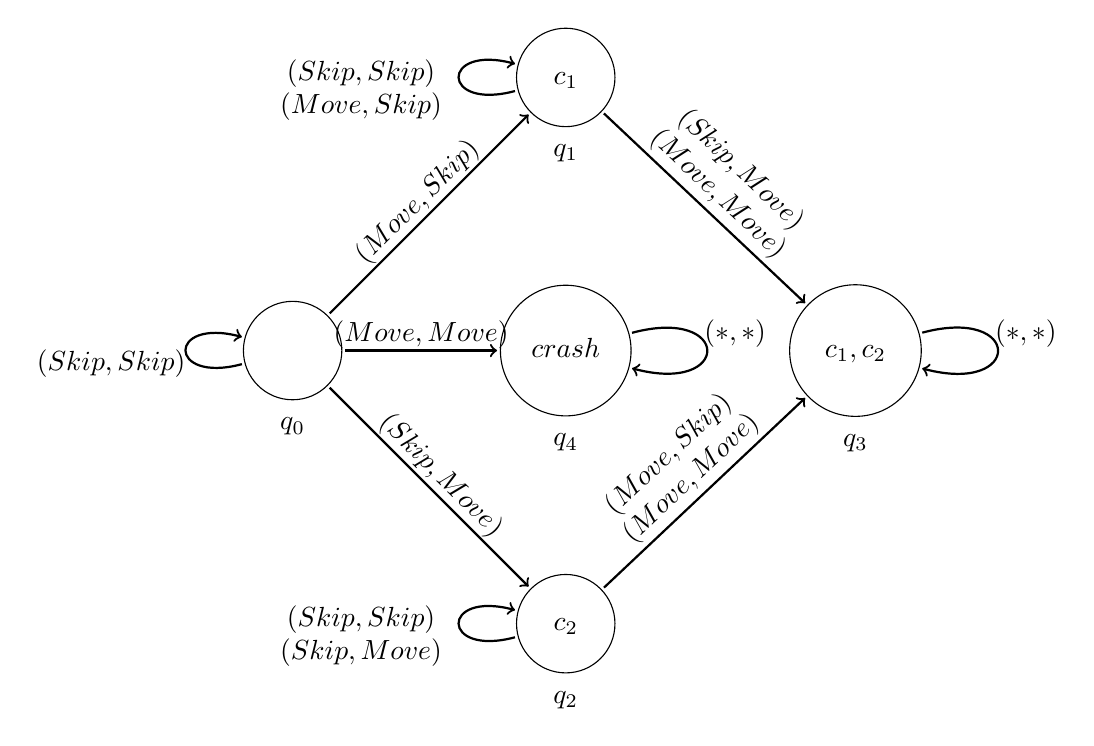
\begin{tikzpicture}[shorten >= 1pt, shorten <= 1pt,  auto]
  \tikzstyle{rond}=[circle,draw=black,minimum size  = 1.25cm] 
   \tikzstyle{label}=[sloped,shift={(0,-.1cm)}]
  
  \node[rond,fill=white] (q0) { \begin{tabular}{c}   \end{tabular}};
  %\node[below=0.1cm of q0]{$init$};
  \node[rond,fill=white] (q4) [right= 2cm of q0] {\begin{tabular}{c} $crash$  \end{tabular}};
  \node[rond,fill=white] (q2) [ below= 2cm   of q4] {\begin{tabular}{c} $c_2$  \end{tabular}};
   \node[rond,fill=white] (q1) [ above= 2cm  of q4] {\begin{tabular}{c} $c_1$   \end{tabular}}; 
  \node[rond,fill=white,mystyle] (q3) [ right= 2cm  of q4] {\begin{tabular}{c} $\begin{tabular}{c} $c_1,c_2$\end{tabular}%w_3
  $  \end{tabular}};


  \node  [below= 0.1cm  of q0] {$q_0$};
  \node  [below= 0.1cm  of q1] {$q_1$};
  \node  [below= 0.1cm  of q2] {$q_2$};
  \node  [below= 0.1cm  of q3] {$q_3$};
  \node  [below= 0.1cm  of q4] {$q_4$};



%bend left= 20, \begin{tabular}{c} $(t,t)/1$ \\  $(t,d)/0.5 $  \end{tabular}
 \path[->,thick] (q0) edge  node [label,pos=.5]    {$(Skip,Move)$}    (q2);
 \path[->,thick] (q2) edge  node [label,pos=.5]    {\begin{tabular}{c} $(Move,Skip)$\\$(Move,Move) $\end{tabular}
 }    (q3);
 \path[->,thick] (q0) edge  node [label,pos=.5]    {$(Move,Skip)$}    (q1);
  \path[->,thick] (q1) edge  node [label,pos=.5]    {\begin{tabular}{c} $(Skip,Move)$\\$(Move,Move) $\end{tabular}
  }    (q3);
 \path[->,thick] (q0) edge  node [label,pos=.5]    {$(Move,Move)$}    (q4);

\path [->,thick] (q0) edge[loop left]  node  [pos=.3]   {$(Skip,Skip)$} (q0);
\path [->,thick] (q2) edge[loop left]  node  [pos=.3]   {\begin{tabular}{c} $(Skip,Skip)$\\$(Skip,Move) $\end{tabular}}  (q2);
\path [->,thick] (q1) edge[loop left]  node  [pos=.3]   {\begin{tabular}{c} $(Skip,Skip)$\\$(Move,Skip) $\end{tabular}}  (q1);
\path [->,thick] (q3) edge[loop right]  node  [pos=.3]   {%\begin{tabular}{c} $(Skip,Skip)$ \\  $(Skip,Move)$\\$(Move,Skip)$ \end{tabular}
$(*,*)$
}  (q3);
\path [->,thick] (q4) edge[loop right]  node  [pos=.3]   {$(*,*)$}  (q4);

\end{tikzpicture}
}

     \caption{Model $M_{cross}$ representing a  system with two vehicles approaching an intersection. 
     Arrows represent transitions between states and are labeled by joint actions of $v_1$ and $v_2$. $(*,*)$ denotes any action.
     } 
     \label{fig:model} 
 \end{figure}

%Formally, $P_{cross} = (M_{cross},\Omega_{M_{cross}})$, where $M_{cross}$ is represented by Figure \ref{fig:model}
%$M_{cross} = ( W,  \ACT,  (\relAct{\jactatm}   )_{\jactatm \in \JACT},  \valProp  )$, $\Omega_M=(\preceq_{i,w }   )_{i \in \AGT, w \in W }$ and
%\begin{itemize}
%    \item $W =\{w_0, w_1, w_2, w_4\}$ 
%    \item $\ACT = \{Move, Skip\}$ 
%    \item $\relAct{(Skip,Skip)} = \{(i,i):i \in W\}$ ; 
%    \item $\relAct{(Skip,Move)} = \{(w_0,w_1),
%    (w_1,w_1),     (w_2,w_3), (w_3, w_3), (w_4,w_4) \}$;  
%    \item $\relAct{(Move, Skip)} = \{(w_0,w_2),
%    (w_1,w_3),     (w_2,w_2), (w_3, w_3), (w_4,w_4) \}$;  
%    \item $\relAct{(Move, Move)} = \{(i,w_4): i \in W \}$;  %->changed this in the figure to no collision after crossing
% \item $ \valProp(w_0)=\emptyset;   \valProp(w_1)=\{crossed_{1}\};     \valProp(w_2)=\{crossed_{2}\};    \valProp(w_3)=\{crossed_{1},crossed_{2}\}; \valProp(w_4)=\{collision\}   $
%\end{itemize}
 %$\preceq_{i,w } $ for each $i \in \AGT, w \in W$  \textcolor{red}{( they prefer paths with "no collision and they crossed" > "no collision", they can also prefer to cross the sooner)}



\end{example}

The following definition introduces the notions
of path and computation, two essential elements of temporal
logics and logics for strategic reasoning.
 \begin{definition}[Path and computation]
A \emph{path}
in a  CGS
$M = ( W,  \ACT,  \relActJoint,  \valProp  )$ is a sequence
$\lambda= w_0 w_1 w_2 \ldots$
of states from  $W$ 
 such that
$w_k    \relAct{ } w_{k +1 }$
for all $k \geq 0$,
    where we recall $\relAct{ }   = \bigcup_{  \jactatm \in \JACT }  \relAct{  \jactatm}$. 
The set of all paths in $M$ is denoted by  $\pathset_M$.
Given a path $\lambda$
of length higher than $k'$ and $k\leq k'$,
the $k$-th element of $\lambda$
is denoted by $\lambda(k)$. 
A \emph{computation}  (or  \emph{full path})
in $M$
is a path $\lambda \in \pathset_M$
such that there is no $\lambda' \in \pathset_M$ of which $\lambda $ is a proper prefix.
The set of all computations in $M$ is denoted  by $\historyset_M$.
The set of all computations in $M$
starting at world $w \in W$ 
(i.e., whose first element is $w$) 
is denoted by  $\historyset_{M,w}$.
\end{definition}

From Constraint C3 in Definition \ref{CGS}, 
it is easy to prove the following fact. 
\begin{fact}
    If $\lambda \in\historyset_M $
    then $\lambda$
    is infinite.
\end{fact}

%%Due to Constraint C3 in Definition 1 (i.e., seriality), a computation can be explicitly defined as an infinite path without using the notion of proper prefix. The current definition of computation given in Definition 2 works even without Constraint C3. 

An agent's individual 
perfect recall
strategy is nothing
but the specification
of a choice for the agent at the end
of every finite path 
in a CGS. 
It is formally defined as follows. 

\begin{definition}[Individual strategy]
Let $M = ( W,  \ACT,  \relActJoint,  \allowbreak \valProp  )$
be a CGS. A (perfect recall) strategy for agent  $i$
    in $M$
    is a function $\strategy_i   $
    that maps every
    finite path $w_0 \ldots w_k\in 
    \pathset_{M }$
    to a choice $\strategy_i(w_0 \ldots w_k) \in \choiceSet_i( w_k )$
    available to agent $i$
    at the end of this finite path,
    where again  we recall $\relAct{ }   = \bigcup_{  \jactatm \in \JACT }  \relAct{  \jactatm}$.
\end{definition}



A collective  strategy   is the assignment of an individual
strategy to each agent. 


\begin{definition}[Collective strategy]
Let $M = ( W,  \ACT, \relActJoint, \allowbreak \valProp  )$
be a CGS. 
A collective strategy   for a  coalition $\Group$
in $M $
     is a function $\strategymap_\Group$
     that associates every agent $i \in \Group$
     to a strategy $\strategymap_\Group(i)$
     for $i$ in $M$. 
     The set of collective  strategies for coalition
      $\Group$ in $M$ is denoted by  $\stratsetatl_{M}^\Group $.
      Its elements are denoted by 
      $\strategymap_\Group , \strategymap_\Group', \ldots $
%      We write
%        $\strategy$ instead of $\strategy_\AGT$,
%        and
%  $\stratsetatl$ instead of  $\stratsetatl_\AGT$.
%For terminological convenience, 
%elements of $\stratsetatl_{M}^\AGT $
%are called complete (collective)  strategies. 
%We define 
% $\stratsetatl_{M}= \bigcup_{\Group \subseteq \AGT }\stratsetatl_{M}^\Group $
%to be the set of all collective  strategies in $M$
%and note $\strategymap, \strategymap', \ldots $ its elements.
%Given an arbitrary  collective strategy
%$\strategymap \in \stratsetatl_{M} $
%we note $\mathit{dom}(\strategymap)$
%its domain. 
\end{definition}


Given a coalition $\Group$, 
$\strategymap_\Group \in \stratsetatl_{M}^\Group $
and 
$\strategymap_{\AGT \setminus \Group}' \in \stratsetatl_{M}^{\AGT \setminus \Group} $,
we define 
$\strategymap_\Group 
\oplus 
\strategymap_{\AGT \setminus \Group}'
\in \stratsetatl_{M}^{\AGT } 
$ to be the composition of the two strategies:
\begin{align*}
&\strategymap_\Group 
\oplus 
\strategymap_{\AGT \setminus \Group}'(i)=
\strategymap_\Group (i) \text{ if }i \in \Group,\\
&\strategymap_\Group 
\oplus 
\strategymap_{\AGT \setminus \Group}'(i)=
\strategymap_{\AGT \setminus \Group}'(i) \text{ otherwise}.
\end{align*}

%\circ to \oplus

Given an initial
state $w$ and a  collective strategy  for
a coalition 
  $\Group$
  we can compute the set of computations generated by
  this strategy
  starting at $w$.

\begin{definition}[Generated computations]
Let $M = ( W,  \ACT, $ $ \relActJoint,  \valProp  )$
be a CGS,
$w\in W$
and $\strategymap_\Group \in \stratsetatl_{M}^\Group  $. 
The set 
$\outset_M(w, \strategymap_\Group)$
denotes
the
set of all computations
$\lambda = w_0 w_1 w_2 \ldots $
in $\historyset_{M}$
such that
$w_0=w$
and
for every $k \geq 0$,   there is $ \jactatm \in \JACT  $ such that:
\begin{itemize}
%\item
%$\relAct{ \jactatm  } (w_k ) \neq \emptyset$,
\item $\strategymap_\Group (i)(w_0 \ldots w_k) =  \jactatm(i) $
for all $i \in \Group$, and 
\item $ w_k  \relAct{ \jactatm  } w_{k +1  }$. 
\end{itemize}

 


\end{definition}

$\outset_M(w, \strategymap_\Group)$
is
the set of computations in  $M$
generated by 
coalition $\Group$'s
collective strategy 
$\strategymap_\Group$
starting at state $w$. 
 Note that
the set $\outset_M (w, \strategymap_\AGT )$
is a singleton 
because of 
Constraint C1  
for collective choice  determinism. 
The unique element of 
$\outset_M (w, \strategymap_\AGT )$
is denoted by $\lambda^{M{,}w{,}\strategymap_\AGT }$.

Note also that there is a single strategy 
$\strategymap_\emptyset $
for the empty coalition, the one which
makes no assignments at all.
Thus, 
$\outset_M (w, \strategymap_\emptyset  )=\historyset_{M,w}$. 

\subsection{Adding preferences}
\label{sec:pref}

In this section,
we extend the notion
of CGS of Definition \ref{CGS}
with preferences.
 \begin{definition}[CGS with preferences]\label{def:cgspref}
 Let 
 $M = ( W,  \ACT,  \allowbreak \relActJoint, 
  \valProp  )$
  be a CGS. A preference structure for $M$
  is a tuple $\Omega_M=(\preceq_{i,w }   )_{i \in \AGT, w \in W }$
  where, for every $i \in \AGT$ and $w \in W$, 
  $\preceq_{i,w }$
  is total preorder over $  \historyset_{M,w}$.
  We call the pair $(M,\Omega_M)$
  a CGS with preferences (CGSP). 
  As usual, we write 
    $\lambda' \prec_{i,w } \lambda$
    if 
       $\lambda' \preceq_{i,w } \lambda$
       and
          $\lambda \not \preceq_{i,w } \lambda'$.
          % The class of CGSPs is denoted
          % by $\classcgsp$.
          
          We say that the CGSP 
          $(M,\Omega_M)$ has stable preferences
          if
          the following condition holds:
          \begin{align*}
       (\mathbf{SP}) \   \forall w,v \in W ,
          \forall \lambda, \lambda' \in 
          \historyset_{M,v },
          & \text{ if } w \relAct{ }  v
          \\ &
          \text{ then }
          \big(
        \lambda'   \preceq_{i,v}\lambda  \text{ iff }
        w  \lambda'   \preceq_{i,w } w\lambda 
          \big). 
          \end{align*}
\end{definition}
Constraint $ \mathbf{SP}$
for stable preferences captures the fact
that an agent's preference is stable over time:
an agent prefers a computation $\lambda $ to a computation $\lambda '$ 
starting  at  the same world  $v$ 
if and only if it prefers the precursor  of $\lambda$
(i.e., $w \lambda $)
to the precursor of $\lambda '$ 
(i.e., $w \lambda'  $)
at each
predecessor $w$ of $v$. 




\begin{example}[Crossing road (cont.)]
Let us resume our example. 
The preference relations $\preceq_{v_1,w_0}$ and $\preceq_{v_2,w_0}$ of agents $v_1$ and $v_2$ (resp.) in state $w_0$ is illustrated in Figure \ref{fig:pref} (preference relation over the other states are analogous). 
The intuition of the preference of each agents $v_i$ is that the less preferred situation for each agent is when there is a collision (the computation indicated with $-_i$). 
Additionally, the agents prefer computations in which he crossed (indicated by %$++$ and
$+_i$) to the ones he did not ($=_i$). 
%Finally, the agent prefers to cross before the agent $v_2$ (computations indicated with $++$). 
We denote by
$P_{cross} = (M_{cross},\Omega_{M_{cross}})$ the CGS $M_{cross}$ with preferences 
$\Omega_M=(\preceq_{i,w } )_{i \in \AGT, w \in W }$.




\begin{figure}[h]

   \centering

     \scalebox{.7}{
     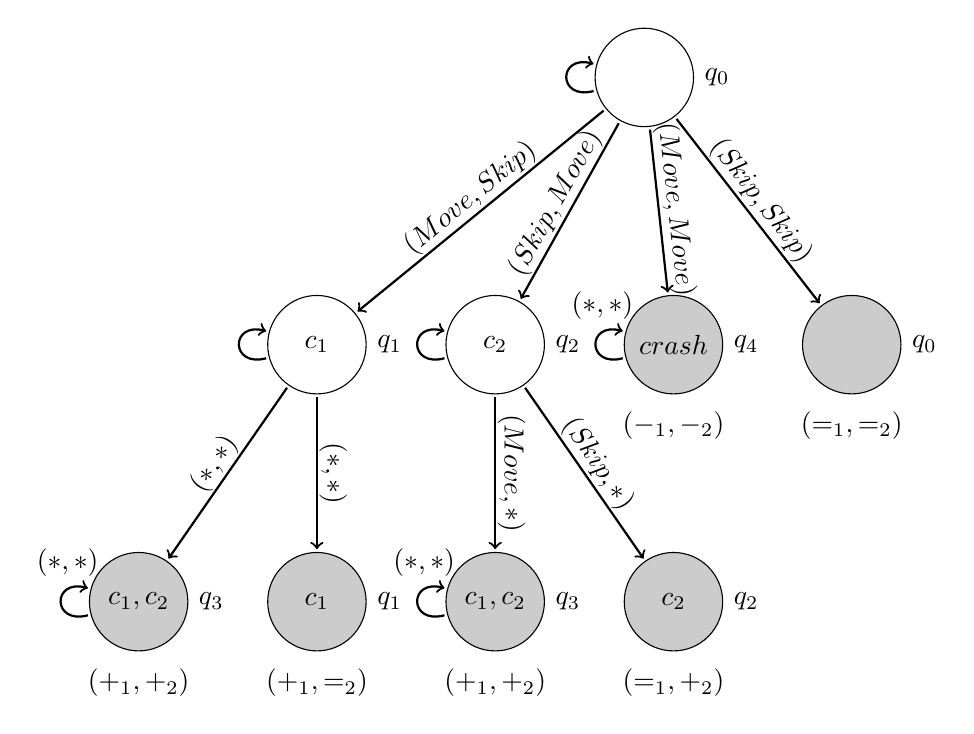
\begin{tikzpicture}[shorten >= 1pt, shorten <= 1pt,  auto]
  \tikzstyle{rond}=[circle,draw=black,minimum size  = 1.25cm] 
   \tikzstyle{label}=[sloped,shift={(0,-.1cm)}]
  
  \node[rond,fill=white] (q0) {};

  %2nd level
  \node[rond,fill=white] (q1) [below left= 2.5cm and 1cm of q0] { $c_2$};
  \node[rond,fill=white] (q2)  [left= 1cm of q1] {$c_1$};
  \node[rond,mystyle,fill=black!20] (q3)  [right= 1cm of q1] {$crash$};
  \node[rond,fill=black!20] (q4) [right= 1cm of q3]  { };
  \path[->,thick] (q0) edge  node [label,pos=.5]    {$(Skip, Move)$}    (q1);
  \path[->,thick] (q0) edge  node [label,pos=.5]    {$(Move, Skip)$}    (q2);
  \path[->,thick] (q0) edge  node [label,pos=.5]    {$(Move, Move)$}    (q3);
  \path[->,thick] (q0) edge  node [label,pos=.5]    {$(Skip, Skip)$}    (q4);
  \path [->,thick] (q3) edge[loop left,looseness=4]  node  [pos=.5,xshift=.6cm, yshift=0.5cm
  ]   {$(*,*)$}  (q3);
  %\path [->,dotted,thick,bend right] (q4) edge  node [label,pos=.5]    {}  (q0);
  \path [->,%dotted,
  thick] (q0) edge[loop left,looseness=4]  node [label,pos=.5]    {}  (q0);
  
  
  %3rd level
  \node[rond,fill=black!20] (q6)  [below= 2cm of q2] {$c_1$};
  \node[rond,mystyle,fill=black!20] (q5)  [left= 1cm of q6]   {$c_1,c_2$};
  \path[->,thick] (q2) edge  node [label,pos=.5]    {$(*,*)$}    (q6);
  \path[->,thick] (q2) edge  node [label,pos=.5]    {$(*,*)$}    (q5);
  \path [->,thick] (q5) edge[loop left,looseness=4]  node  [pos=.5,xshift=.6cm, yshift=0.5cm]   {$(*,*)$}  (q5); 
 % \path [->,dotted,thick,bend right] (q6)
  edge  node [label,pos=.5]    {}  (q2);
  \path [->,%dotted,
  thick] (q2) edge[loop left,looseness=4]  node [label,pos=.5]    {}  (q2);


  \node[rond,mystyle,fill=black!20] (q7)  [below= 2cm of q1] {$c_1,c_2$};
  \node[rond,mystyle,fill=black!20] (q8)  [right= 1cm of q7]   {$c_2$};
  \path[->,thick] (q1) edge  node [label,pos=.5]    {$(Move, *)$}    (q7);
  \path[->,thick] (q1) edge  node [label,pos=.5]    {$(Skip, *)$}    (q8);
  \path [->,thick] (q7) edge[loop left,looseness=4]  node  [pos=.5,xshift=.6cm, yshift=0.5cm]   {$(*,*)$}  (q7);
  %\path [->,dotted,thick,bend right] (q8) 
   edge  node [label,pos=.5]    {}  (q1);
   \path [->,%dotted,
   thick] (q1) edge[loop left,looseness=4]  node [label,pos=.5]    {}  (q1);


  \node  [right= 0.01cm  of q0] {$q_0$};
  \node  [right= 0.01cm  of q4] {$q_0$};

  \node  [right= 0.01cm  of q2] {$q_1$};
  \node  [right= 0.01cm  of q6] {$q_1$};

  \node  [right= 0.01cm  of q1] {$q_2$};
  \node  [right= 0.01cm  of q8] {$q_2$};
  
  \node  [right= 0.01cm  of q5] {$q_3$};
  \node  [right= 0.01cm  of q7] {$q_3$};

  \node  [right= 0.01cm  of q3] {$q_4$};

  \node[below=0.1cm of q5]{$(+_1,+_2)$}; %c1,c1c2 %++
  \node[below=0.1cm of q6]{$(+_1,=_2)$}; %loop c1
  \node[below=0.1cm of q7]{$(+_1,+_2)$};%c2,c1c2
  \node[below=0.1cm of q8]{$(=_1,+_2)$};%c2,
  \node[below=0.1cm of q4]{$(=_1,=_2)$};%init,
  \node[below=0.1cm of q3]{$(-_1,-_2)$};%init,

  %\node[rond,fill=white,mystyle] (q) [ right= 2cm  of q4] {$c_1,c_2$};
 

%bend left= 20, \begin{tabular}{c} $(t,t)/1$ \\  $(t,d)/0.5 $  \end{tabular}
% \path[->,thick] (q0) edge  node [label,pos=.5]    {}    (q1);
 
%\path [->,thick] (q4) edge[loop right]  node  [pos=.3]   {}  (q4);

\end{tikzpicture}
}

     \caption{Representation of the unravelling of $M_{cross}$ from the initial state ($w_0$). Branches represent (groups of) computations. Transitions are labeled by the action taken by $v_1$ and $*$ denotes any action. Self-loops indicate computations where the state is repeated. %Dotted arrows indicate computations that repeat in a given state but may proceed to a different state.
     %preference relations $\preceq_{v_1,w_0}$ and $\preceq_{v_2,w_0}$ 
     Grey states indicate computations with an infinite suffix that repeats on the same state. Labels in the form under the grey states represent the preference relations  $\preceq_{v_1,w_0}$ and $\preceq_{v_2,w_0}$  of the agents $v_1$ and $v_2$, respectively.  Computations labeled with $+_i$ are strictly  preferred to $=_i$ by agent $v_i$, and  $=_i$ are strictly preferred to~$-_i$ by agent $v_i$ (where $i = \{1,2\}$).     } 
     \label{fig:pref} 
 \end{figure}


The strategies in which the agent performs $Move$ in the initial state are not dominated, because it may lead to the state where he crossed or to a collision. 
On the other hand, the strategy in which the agent waits (action $Skip$) when only the other agent has crossed is dominated by the strategy in which he moves whenever agent $v_2$ has crossed.   
\end{example}


The following definition introduces
the notion 
of dominated strategy,
the essential constituent 
of minimal rationality
for agents. 
 \begin{definition}[Dominated strategies]
Let $P=(M,\Omega_M)$ be a CGSP
with  $M = ( W,  \ACT,  \relActJoint, 
  \valProp  )$
  a CGS and $\Omega_M=(\preceq_{i,w }   )_{i \in \AGT, w \in W }$
  a preference structure for $M$, 
 $i \in \AGT$, $w \in W$,
  and  $\strategymap_{\{i\}},\strategymap_{\{i\}}' \in \stratsetatl_{M}^{\{i\}}$.
  We say that at world $w$
  agent $i$'s strategy $\strategymap_{\{i\}}' $
  dominates agent $i$'s  strategy $\strategymap_{\{i\}} $
  iff 
  \begin{align*}
  \forall \strategymap_{\AGT \setminus {\{i\}}}''
    \in \stratsetatl_{M}^{\AGT \setminus {\{i\}} },
 \lambda^{M{,}w{,}\strategymap_{\{i\}}   \oplus 
 \strategymap_{\AGT \setminus {\{i\}} }''}  
 \prec_{i,w}  \lambda^{M{,}w{,}\strategymap_{\{i\}}'  \oplus 
 \strategymap_{\AGT \setminus {\{i\}}}''}  . 
  \end{align*}
  Agent $i$'s strategy $\strategymap_{\{i\}} $
    is said to be dominated at $w$ 
    if
    there exists another strategy $\strategymap_{\{i\}} '$
    of $i$
    which dominates $\strategymap_{\{i\}} $  at $w$.
 Agent $i$'s set of dominated strategies
  at $w$ 
  is denoted by $\mathit{Dom}_{M,w}^i$.
  % Conversely, $\mathit{Undom}_{M,w}^i$
  %  is  agent $i$'s set of non-dominated strategies
  % at $w$. 
\end{definition}

In the next section
we introduce 
a novel
language
that extends
the language
of $\atllogic$
with a family of operators
for rational capability.
It will be  interpreted by means
of the notion of CGSP. 


 
 
\section{Language }\label{sec:language}
 

The language of $\atlratlogic$
($\atllogic$ with \emph{minimal rationality}), denoted 
by $\lang_{\atlratlogic}(\ATM, \AGT )$,
is defined by the following grammar: 
\begin{center}\begin{tabular}{lcl}
 $\varphi, \psi$  & $\bnf$ & $p \mid \neg\varphi \mid \varphi \wedge \psi  \mid
 \atlop{\Group}
\nexttime \varphi \mid 
 \atlop{\Group}
\henceforth  \varphi 
 \mid   \atlop{\Group}
 (\until{\varphi}{\psi} )$\\
 &  & $ \atloprat{\Group}
\nexttime \varphi \mid 
 \atloprat{\Group}
\henceforth  \varphi 
 \mid   \atloprat{\Group}
 (\until{\varphi}{\psi} ),$
\end{tabular}\end{center}
where  $p$
ranges over  $\ATM$
and $\Group $ ranges over $2^\AGT$. 
The other Boolean connectives
and constructs 
$\vee, \rightarrow, \leftrightarrow, \top, \bot $
are defined as abbreviations in the usual way.

On the one hand, 
formulas 
$  \atlop{\Group}
\nexttime \varphi$,
$  \atlop{\Group}\henceforth \varphi  $
and 
$  \atlop{\Group}( \until { \varphi    } { \psi    }) $
capture the notion of strategic  capability.
They 
have the usual
$\atllogic$ readings:
$  \atlop{\Group}
\nexttime \varphi$
has to be read 
``coalition $\Group$ has 
a strategy at its disposal 
which guarantees that
$\varphi$ is going to be true in the next state'',
while 
$  \atlop{\Group}\henceforth \varphi  $
has to be read 
``coalition $\Group$ has 
a strategy at its disposal 
which guarantees that   
 $\varphi$ will always be true''. 
Finally, 
$  \atlop{\Group}( \until { \varphi    } { \psi    }) $
has to be read 
``coalition $\Group$ has 
a strategy at its disposal 
which guarantees that   
 $\varphi$ will be true until $\psi$ is true''.
 On the other hand,
 formulas 
 $  \atloprat{\Group}
\nexttime \varphi$,
$  \atloprat{\Group}\henceforth \varphi  $
and 
$  \atloprat{\Group}( \until { \varphi    } { \psi    }) $
capture the notion
of \emph{rational} strategic capability: 
$  \atloprat{\Group}
\nexttime \varphi$
has to be read 
``coalition $\Group$ has 
a \emph{rational} strategy at its disposal 
which guarantees that
$\varphi$ is going to be true in the next state'',
$  \atloprat{\Group}\henceforth \varphi  $
has to be read 
``coalition $\Group$ has 
a \emph{rational} strategy at its disposal 
which guarantees that   
 $\varphi$ will always be true''. 
Finally, 
$  \atloprat{\Group}( \until { \varphi    } { \psi    }) $
has to be read 
``coalition $\Group$ has 
a \emph{rational} strategy at its disposal 
which guarantees that   
 $\varphi$ will be true until $\psi$ is true''. 
 

Formulas of the language 
$\lang_{\atlratlogic}(\ATM, \AGT )$
are evaluated relative to a pair   
$(P,w)$
with 
$P=(M,\Omega_M)$
a CGSP, 
 $M = ( W,  \ACT,  \allowbreak \relActJoint, 
  \valProp  )$
  a CGS,
  $\Omega_M$
  a preference structure for $M$
  and $w \in W$, as follows:
 \begin{eqnarray*}
   (P,w ) \models   p  & \Longleftrightarrow  &  
  p\in    \valProp\big(\lambda(0) \big)
 ,\\
  (P,w ) \models   \atlop{\Group}
 \nexttime \varphi  & \Longleftrightarrow  &  
  \exists \strategymap_\Group \in  \stratsetatl^\Group_M
  \text{ s.t. }\forall \lambda \in \outset(w, \strategymap_\Group),
  \\ & &
\big( P, \lambda(1)  \big)\models \varphi ,\\
  (P,w ) \models   \atlop{\Group}
 \henceforth  \varphi  & \Longleftrightarrow  &  
  \exists \strategymap_\Group \in  \stratsetatl^\Group_M
  \text{ s.t. }\forall \lambda \in \outset(w, \strategymap_\Group),\\
&& \forall k > 0, \big( P, \lambda(k)  \big)\models \varphi ,\\
(   P,w)\models  \atlop{\Group}( \until { \varphi    } { \psi    })
     & \Longleftrightarrow  &  
   \exists  \strategymap_\Group
  \in \stratsetatl^\Group_M \text{ s.t. }
   \forall  \lambda \in \outset(w, \strategymap_\Group) , \\
   && \exists k > 0 \text{ s.t. } \big(  P,\lambda(k) \big)  \models \psi \text{ and } \\
&& \forall 
   h \in \{ 1, \ldots, k-1\}  , \big( P, \lambda(h) \big) \models \varphi ,\\
     (P,w ) \models   \atloprat{\Group}
 \nexttime \varphi  & \Longleftrightarrow  &  
  \exists \strategymap_\Group \in  \stratsetatl^\Group_M
  \text{ s.t. }
  \forall i \in \Group, 
   \\ & & \strategymap_\Group|_{\{i\}}\not \in \mathit{Dom}_{M,w}^i \text{ and }\\
 && \forall \lambda \in \outset(w, \strategymap_\Group),
\big( P, \lambda(1)  \big)\models \varphi ,\\
  (P,w ) \models   \atloprat{\Group}
 \henceforth  \varphi  & \Longleftrightarrow  &  
  \exists \strategymap_\Group \in  \stratsetatl^\Group_M
  \text{ s.t. }   \forall i \in \Group, 
   \\ & & \strategymap_\Group|_{\{i\}}\not \in 
  \mathit{Dom}_{M,w}^i \text{ and } \\
  && \forall \lambda \in \outset(w, \strategymap_\Group),\\
&& \forall k > 0, \big( P, \lambda(k)  \big)\models \varphi ,\\
(   P,w)\models  \atloprat{\Group}( \until { \varphi    } { \psi    })
     & \Longleftrightarrow  &  
   \exists  \strategymap_\Group
  \in \stratsetatl^\Group_M \text{ s.t. }
    \forall i \in \Group, \\
    &&
    \strategymap_\Group|_{\{i\}}\not \in \mathit{Dom}_{M,w}^i \text{ and }\\
&&   \forall  \lambda \in \outset(w, \strategymap_\Group) , \\
   && \exists k > 0 \text{ s.t. } \big(  P,\lambda(k) \big)  \models \psi \text{ and } \\
&& \forall 
   h \in \{ 1, \ldots, k-1\}  , \big( P, \lambda(h) \big) \models \varphi ,
\end{eqnarray*}
where $ \strategymap_\Group|_{\{i\}}$
is the restriction
of function
$\strategymap_\Group$
to $\{i\}\subseteq \Group$.
Note that the difference between
the strategic capability
operators
and the \emph{rational}
strategic capability
operators
lies in the restriction
to non-dominated (minimally rational)
strategies. 
While the  $\atllogic$
strategic capability 
operators existentially quantify
over
the set of collective strategies 
of the coalition $\Group$ (i.e., $  \exists \strategymap_\Group \in  \stratsetatl^\Group_M$),
their  rational  
counterparts
existentially
quantify 
over
the set of collective strategies 
of the coalition $\Group$
such that all 
their individual
components  are not dominated
(i.e., $\forall i \in \Group, 
    \strategymap_\Group|_{\{i\}}\not \in 
  \mathit{Dom}_{M,w}^i$).
 

The following fragment 
defines 
the language of $\clratlogic$
($\cllogic$ with \emph{Minimal Rationality}), denoted
by $\lang_{\clratlogic}(\ATM, \AGT )$: 
\begin{center}\begin{tabular}{lcl}
 $\varphi, \psi$  & $\bnf$ & $p \mid \neg\varphi \mid \varphi \wedge \psi  \mid
 \atlop{\Group}
\nexttime \varphi \mid  \atloprat{\Group}
\nexttime \varphi, $
\end{tabular}\end{center}
where  $p$
ranges over  $\ATM$
and $\Group $ ranges over $2^\AGT$. 

The languages $\lang_{\atllogic}(\ATM, \AGT )$ of $\atllogic$
and $\lang_{\cllogic}(\ATM, \AGT )$ of $\cllogic$
are defined as usual:
\begin{itemize}
    \item
    $\lang_{\atllogic}(\ATM, \AGT )$ is the fragment of
$\lang_{\atlratlogic}(\ATM, \AGT )$
with no formulas
 $\atloprat{\Group}
\nexttime \varphi ,
 \atloprat{\Group}
\henceforth  \varphi 
,   \atloprat{\Group}
 (\until{\varphi}{\psi} )$, and
 \item 
  $\lang_{\cllogic}(\ATM, \AGT )$ is the fragment of
$\lang_{\clratlogic}(\ATM, \AGT )$
with no formulas
 $\atloprat{\Group}
\nexttime \varphi$.
\end{itemize}


 

 \begin{example}[Crossing road (cont.)]
%\textcolor{red}{WIP}  
 
 Returning to our example, it is easy to check that 
 $(P_{croos}, w_0) \models \atloprat{v_1} \nexttime \neg crash  
 $ 
 that is, agent $v_1$ has a rational strategy to avoid a collision. 
However, the agent $v_1$ has no rational strategy to ensure to \textit{eventually} cross the street, that is, 
$(P_{croos}, w_0) \not \models  \atloprat{v_1}  \top \untill c_1 
 $.

 \end{example}






\section{Tree-like  model property and embedding }\label{sec:resultsblock}

In this section we first  state
the tree-like model property for the language $\lang_{\atlratlogic}(\ATM, \AGT )$.
Thanks to it, we will provide 
a polynomial embedding
of the $\atlratlogic$-language
into the 
$\atllogic$-language
which also offers  a polynomial embedding of 
the
 $\clratlogic$-language
into the
$\cllogic$-language.
Thanks to the embedding 
we will be able
to provide tight complexity results
for satisfiability checking for the 
two languages $\lang_{\atlratlogic}(\ATM, \AGT )$
and
$\lang_{\clratlogic}(\ATM, \AGT )$. 



\subsection{Tree-like  model property}


Let
 $\relAct{ }^*$, $\relAct{ }^-$ and $\relAct{ }^+$
be, respectively, the reflexive and  transitive closure,
the inverse, and the transitive closure of 
$\relAct{ } = \bigcup_{  \jactatm \in \JACT }  \relAct{  \jactatm}$.
\begin{definition}\label{def:propertiesCGS}
  Let $M = ( W,  \ACT,   \relActJoint,  \valProp  )$
  be a CGS.
  We say that:
  \begin{itemize}
    \item $M$ has a unique root iff
          there is  a unique $ w_0 \in W$ (called the \emph{root}),
          such that, for every $v \in W$, $w_0 \relAct{ }^* v$;
    \item $M$ has unique predecessors iff
          for every $v \neq w_0 $, the cardinality of $\relAct{ }^-( v)$ is at most one;
    \item $M$ has no cycles iff $\relAct{ }^+$ is irreflexive;


    \item $M$ is tree-like iff  it has a unique root,
 unique predecessors and no cycles;

     \item $M$
    is joint action disjoint iff for every $w \in W$
    and for every $\jactatm, \jactatm' \in \JACT $,
    if $\jactatm\neq \jactatm'$
    then $ \relAct{\jactatm} (w) \cap \relAct{\jactatm' } (w) =\emptyset$.
    
  \end{itemize}




\end{definition}

The 
property of 
``having stable preferences''
defined in Definition \ref{def:cgspref}
and the 
properties of ``having unique root'',
``having unique predecessors'',
``having no cycles'',
``being tree-like''
and ``being joint action disjoint''
defined in %the previous
Definition \ref{def:propertiesCGS}
are abbreviated $\mathit{sp},\mathit{ur},\mathit{up} ,
\mathit{nc}, \allowbreak \mathit{tr}$ and $ \mathit{ad} $. 
  The properties defined in %the previous
  Definition \ref{def:propertiesCGS}
  naturally extend to CGSPs: the CGSP
  $P=(M,\Omega_M)$ satisfies one of these properties 
  if the underlying CGS $M$
  satisfies it.  
  For every $X\subseteq \{\mathit{sp}, \mathit{ur},\mathit{up} ,
\mathit{nc}, \mathit{tr}, \allowbreak \mathit{ad}  \}$,
the class of CGS satisfying the properties in $X$
is denoted by $\classcgspvar{X}$. 
%New
By $\classcgspvar{\emptyset}$, we denote the class of all CGSP.


The following Lemma 
\ref{lemmacrucial}
is a tree-like model property for the language $\lang_{\atlratlogic}(\ATM, \AGT )$.
      The proof of the lemma 
     is given in Appendix A in the supplementary material. 
     The proof relies on a three-step transformation. First, we transform
     a CGSP into a CGSP with joint action disjointness by constructing
     one copy of a state for each possible joint action. Second, we transform
     the resulting CGSP with joint action disjointness into a CGSP with joint action disjointness, unique
     predecessor and no cycles. This second transformation associates every state
     of the original CGSP to a finite path. Third, we generate the submodel
     from the point of evaluation of the original model
     to guarantee unique rootness. 
\begin{lemma}\label{lemmacrucial}
  Let $\varphi \in \lang_{\atlratlogic}(\ATM, \AGT )$.
  Then,
  \begin{itemize}
      \item $\varphi$
      is satisfiable 
      for the class $\classcgspvar{\emptyset } $
      iff  $\varphi$
      is satisfiable 
      for the class $\classcgspvar{\{ \mathit{tr},\mathit{ad}  \}}$,

      \item $\varphi$
      is satisfiable 
      for the class $\classcgspvar{\{\mathit{sp}  \}}$
      iff  $\varphi$
      is satisfiable 
      for the class $\classcgspvar{\{ \mathit{sp},\mathit{tr},\mathit{ad}  \}}$. 
  \end{itemize}
  
   
\end{lemma}
 


\subsection{Embedding}

Let us consider 
the following translation
$\mathit{tr}:
\lang_{\atlratlogic}(\ATM, \AGT ) \longrightarrow
\lang_{\atllogic}(\ATM^+, \AGT )
$ 
with $\ATM^+ =\ATM\cup  \big\{ \mathit{rat}_i \suchthat
i \in \AGT 
\big\}$:
\begin{align*}
  \mathit{tr}(p ) &= p,\\
\mathit{tr}(\neg \varphi  ) &= \neg \mathit{tr}( \varphi  ),\\
\mathit{tr}( \varphi \wedge
\psi ) &=   \mathit{tr}( \varphi  ) \wedge \mathit{tr}( \psi   ) ,\\
\mathit{tr}( \atlop{\Group}
\nexttime \varphi ) &=  \atlop{\Group} \nexttime \mathit{tr}( \varphi  )  ,\\
\mathit{tr}( \atlop{\Group}
\henceforth \varphi ) &=  \atlop{\Group}\henceforth \mathit{tr}( \varphi  ),\\
\mathit{tr}\big( \atlop{\Group}
(\until{\varphi}{\psi})  \big) &=  \atlop{\Group} \big(\until{\mathit{tr}(\varphi)}{\mathit{tr}(\psi)}  \big),\\
\mathit{tr}( \atloprat{\Group}
\nexttime \varphi ) &=  \atlop{\Group} \nexttime
\big(\mathit{rat}_C \wedge \mathit{tr}( \varphi  )\big)  ,\\
\mathit{tr}( \atloprat{\Group}
\henceforth \varphi ) &=  \atlop{\Group}\henceforth \big(\mathit{rat}_C \wedge \mathit{tr}( \varphi  )\big),\\
\mathit{tr}\big( \atloprat{\Group}
(\until{\varphi}{\psi})  \big) &=  \atlop{\Group}\big(
\until{
(\mathit{rat}_C \wedge \mathit{tr}(\varphi) )}
{(\mathit{rat}_C \wedge \mathit{tr}(\psi) ) } \big)  ,
\end{align*}
 with $\mathit{rat}_C\eqdef \bigwedge_{i \in \AGT}  \mathit{rat}_i$
 and the special atomic formula 
 $\mathit{rat}_i$
 standing for ``agent $i$
 is rational''. 


The idea of the translation
is to transform 
a rational capability
operator
into its 
ordinary capability
counterpart using the special
atomic formulas 
$\mathit{rat}_i$. Specifically, the fact that
a coalition $\Group$
has a rational strategy to ensure a given outcome 
is translated into the fact that 
the coalition $\Group$
has a strategy
to force the  outcome 
by ensuring that all its members are rational.
As the following theorem highlights,
satisfiability
of $\atlratlogic$-formulas
is 
reducible to 
satisfiability
of $\atllogic$-formulas
using 
the translation 
$  \mathit{tr}$.
      The proof of the theorem
     is given in Appendix B in the supplementary material.
     The proof relies on a  non-trivial
     construction which 
     transforms
     a tree-like CGSP into a new tree-like  CGSP
     in which an atomic formula of type $   \mathit{rat}_i$
     matches 
     the computations that are generated by a 
     non-dominated strategy  of agent $i$.
     The assumption of stable preferences is essential
     to guarantee that this matching exists. 


     
 \begin{theorem}\label{theo:embedding}
     Let $\varphi \in \lang_{\atlratlogic}(\ATM, \AGT )$.
     Then, 
     $\varphi $
     is satisfiable for  the class 
     $\classcgspvar{\{\mathit{sp} \}}$
     iff $\big( \bigwedge_{i \in \AGT }
     \atlop{ \{i \}} \henceforth  
      \mathit{rat}_i \big)  \wedge
     \mathit{tr}(\varphi) $
     is satisfiable for the class
          $\classcgspvar{\{\mathit{sp} \}}$.
     % \begin{align*}
     %     \models_{\classcgspvar{\{\mathit{sp} \}}} \varphi \text{ iff }
     %  \big\{ \atlop{ \{i \}} \henceforth  
     %  \mathit{rat}_i \suchthat i \in \AGT 
     %  \big\}       \models_{\classcgspvar{\{\mathit{sp} \}}}  \mathit{tr}(\varphi). 
     % \end{align*}
 \end{theorem}
 
 
%   For every $X\subseteq \{\mathit{sp}, \mathit{ur},\mathit{up} ,
% \mathit{nc}, \mathit{tr},\mathit{ad}  \}$,
% the class of CGS satisfying the properties in $X$
% is denoted by $\classcgspvar{X}$. 



 % Deduction theorem:
 % \begin{theorem}
 %     Let $\varphi \in \lang_{\atllogic}(\ATM, \AGT )$
 %     and $\Sigma \subset  \lang_{\atlratlogic}(\ATM, \AGT )$
 %     finite. 
 %     Then, 
 %     \begin{align*}
 %      \Sigma          \models_{\classcgspvar{\{\mathit{sp} \}}}   \varphi 
 %       \text{ iff } 
 %          \models_{\classcgspvar{\{\mathit{sp} \}}}
 %        \atlop{ \emptyset } 
 %                \big( \bigwedge_{\psi \in \Sigma}
 %                \henceforth^* 
 %        \psi  \big) 
 %       \rightarrow \varphi. 
 %     \end{align*}
 % \end{theorem}\

As the following theorem highlights, 
  if we restrict  to the language
$ \lang_{\clratlogic}(\ATM, \AGT )$
the translation $\mathit{tr}$
also  
provides
an  embedding for the general
class
 $\classcgspvar{ }$.
The proof of  Theorem \ref{theo:embedding2}
is a straightforward
adaptation 
of the proof of Theorem \ref{theo:embedding}.
Instead of matching
an atomic formula
  $   \mathit{rat}_i$
  with a computation,
  for every state in a tree-like CGSP
  we match  $   \mathit{rat}_i$ with
  a successor 
  of this state along a computation generated  by a 
     non-dominated strategy  of agent $i$.
 The assumption of stable preferences
 is no longer required
 since the translation
 of formula $ \atloprat{\Group}
\nexttime \varphi $
only refers
to the truth values
of atoms $   \mathit{rat}_i$
in the next state. 

 \begin{theorem}\label{theo:embedding2}
     Let $\varphi \in \lang_{\clratlogic}(\ATM, \AGT )$.
     Then, 
     $\varphi $
     is satisfiable for  the class 
     $\classcgspvar{} $
     iff $\big( \bigwedge_{i \in \AGT }
     \atlop{ \{i \}} \nexttime 
      \mathit{rat}_i \big)  \wedge
     \mathit{tr}(\varphi) $
     is satisfiable for the class
          $\classcgspvar{} $.
     
     % \begin{align*}
     %     \models_{\classcgspvar{\{\mathit{sp} \}}} \varphi \text{ iff }
     %  \big\{ \atlop{ \{i \}} \henceforth  
     %  \mathit{rat}_i \suchthat i \in \AGT 
     %  \big\}       \models_{\classcgspvar{\{\mathit{sp} \}}}  \mathit{tr}(\varphi). 
     % \end{align*}
 \end{theorem}

 
 
The following complexity result
is a direct corollary of Theorems \ref{theo:embedding} and \ref{theo:embedding2},
the fact that the size of $\mathit{tr}(\varphi) $
is polynomial
in the size of the input formula $\varphi$
and the fact that satisfiability checking
for $\atllogic$
is \Exptime-complete \cite{DrimmelenLICS}
and
satisfiability checking
for $\cllogic$
is \Pspace-complete \cite{DBLP:journals/logcom/Pauly02}. 





  \begin{corollary}
Checking satisfiability of
formulas in the language $ \lang_{\atlratlogic}(\ATM, \AGT )$ relative to  the class    $\classcgspvar{\{\mathit{sp} \}}$ 
is  \Exptime-complete.
It is \Pspace-complete
relative to  
both classes   
$\classcgspvar{ } $
and $\classcgspvar{\{\mathit{sp} \}}$, 
when 
restricting to the fragment $ \lang_{\clratlogic}(\ATM, \AGT )$. 
  \end{corollary}



  Before concluding this section,
  we would like to highlight the fact that the translation
  $\mathit{tr}$
  from
  the language $\lang_{\atlratlogic}(\ATM, \AGT )$ to
  the language $\lang_{\atlratlogic}(\ATM^+, \AGT )$
  is adequate 
for  the stable preference
semantics
only. It does not
work for the general
 class $\classcgspvar{}$. 
% works
% the  model class
% $\classcgspvar{\{\mathit{sp} \}}$
% but does not
% work
% for the general
% class
% $\classcgspvar{}$.
% In other words,
% the translation
%   $\mathit{tr}$
% is adequate 
% for  the stable preference
% semantics
% only. 
To see this,
it is sufficient to observe
that, on the one hand, 
the following formula
is valid
for the general 
class 
$\classcgspvar{}$:
\begin{align*}
  \phi_{\Group,p}  =_{\mathit{def}}\atlop{\Group}\henceforth (\mathit{rat}_\Group \wedge p)\to \atlop{\Group}\nexttime \atlop{\Group}\henceforth (\mathit{rat}_\Group \wedge p). 
\end{align*}
Indeed, 
$  \phi_{\Group,p}$
is a basic
validity
of $\atllogic$. 
Moreover, 
we have 
\begin{align*}
\mathit{tr}\big(
\atloprat{\Group}\henceforth p\to \atlop{\Group}\nexttime \atloprat{\Group}\henceforth p
\big) =
\phi_{ \Group,p}. 
\end{align*}
But, on the other hand,
the formula 
$\atloprat{\Group}\henceforth p\to \atlop{\Group}\nexttime \atloprat{\Group}\henceforth p$
is not valid
for the 
class 
$\classcgspvar{}$, 
which is the same thing
as saying that 
$\neg \big( \atloprat{\Group}\henceforth p\to \atlop{\Group}\nexttime \atloprat{\Group}\henceforth p\big) $
is  satisfiable for $\classcgspvar{}$. 
A counter-model
for this formula
is given in Appendix C. % in the supplementary material. 

 Thus,  there is no analog
 of Theorem \ref{theo:embedding}
 for the class
 $\classcgspvar{}$
 since there exists  a formula
 $\varphi $
 (i.e., $\neg \big( \atloprat{\Group}\henceforth p\to \atlop{\Group}\nexttime \atloprat{\Group}\henceforth p\big) $)
which 
 is  satisfiable for
 $\classcgspvar{}$
 and, at the same time, 
 $
 \big( \bigwedge_{i \in \AGT }
      \atlop{ \{i \}} \henceforth 
       \mathit{rat}_i \big)  \wedge
 \mathit{tr}(\varphi)$
is not satisfiable for 
$\classcgspvar{}$
since $\neg  \mathit{tr}(\varphi)$
(i.e., $ \neg \neg \phi_{\Group,p}$
which is equivalent to $  \phi_{\Group,p}$)
is valid
for 
$\classcgspvar{}$.

     % Let $\varphi \in \lang_{\atlratlogic}(\ATM, \AGT )$.
     % Then, 
     % $\varphi $
     % is satisfiable for  the class 
     % $\classcgspvar{\{\mathit{sp} \}}$
     % iff $\big( \bigwedge_{i \in \AGT }
     % \atlop{ \{i \}} \henceforth  
     %  \mathit{rat}_i \big)  \wedge
     % \mathit{tr}(\varphi) $
     % is satisfiable for the class
     %      $\classcgspvar{\{\mathit{sp} \}}$.
  

\section{Axiomatization for $\clratlogic$}\label{axiomatization}
In this section, we first introduce an axiomatic system for $\clratlogic$ and then show its soundness and completeness.

\begin{definition}[Axiomatic system for $\clratlogic$]
\label{definition: axiomatic system for R-CL}
The axiomatic system for $\clratlogic$ consists of the following axioms:
\begin{align}
&  \text{All tautologies of propositional logic} \tag{$\top$} \label{ax:taut} 
\\
&  \neg \atlop{\Group}\nexttime \bot \tag{$\mathtt{A}\text{-}\mathtt{NAAA}$} \label{ax:NAAA} 
\\
& \atloprat{\emptyset } \nexttime \phi \leftrightarrow \atlop{\emptyset } \nexttime \phi \tag{$\mathtt{A}\text{-}\mathtt{NP}_{\emptyset}$} \label{ax:NP}
\\
& 
\atloprat{\Group} \nexttime \phi \to \atlop{\Group } \nexttime \phi \tag{$\mathtt{A}\text{-}\mathtt{MR}$} \label{ax:MR}
\\
& 
\atlop{\emptyset} \nexttime (\phi \to \psi) \rightarrow (\atlop{\Group}\nexttime \phi \rightarrow \atlop{\Group} \nexttime \psi ) \tag{$\mathtt{A}\text{-}\mathtt{MG}0$} \label{ax:MG0}
\\
& 
\atloprat{\emptyset} \nexttime (\phi \to \psi) \rightarrow (\atloprat{\Group}\nexttime \phi \rightarrow \atloprat{\Group} \nexttime\psi) \tag{$\mathtt{A}\text{-}\mathtt{MG}1$} \label{ax:MG1}
\\
&
\atlop{\Group}\nexttime \phi \rightarrow \atlop{\Group'}\nexttime \phi, \text{ for }\Group \subseteq \Group' \tag{$\mathtt{A}\text{-}\mathtt{MC}0$} \label{ax:MC0}
\\ 
& 
\atloprat{\Group}\nexttime \phi \rightarrow \atloprat{\Group'}\nexttime \phi , \text{ for }\Group \subseteq \Group' 
\tag{$\mathtt{A}\text{-}\mathtt{MC}1$} \label{ax:MC1}
\\ 
&
\atlop{\Group}\nexttime \top
\tag{$\mathtt{A}\text{-}\mathtt{NCS}$} \label{ax:Ser}
\\ 
&
(\atlop{\Group} \nexttime \phi \land \atlop{\Group'} \nexttime \psi) \rightarrow   \atlop{\Group \cup \Group'} \nexttime (\phi \land \psi),  \nonumber  \\ & 
\text{ for }\Group \cap \Group' = \emptyset
\tag{$\mathtt{A}\text{-}\mathtt{Sup}0$} \label{ax:Sup0}
\\ 
&
(\atloprat{\Group} \nexttime \phi \land \atloprat{\Group'} \nexttime \psi) \rightarrow \atloprat{\Group \cup \Group'} \nexttime (\phi \land \psi),  \nonumber  \\ &  
\text{ for }\Group \cap \Group' = \emptyset
\tag{$\mathtt{A}\text{-}\mathtt{Sup}1$} \label{ax:Sup1}
\\ 
&
\atlop{\Group} \nexttime (\phi \lor \psi) \rightarrow (\atlop{\Group} \nexttime \phi \lor \atlop{\AGT} \nexttime \psi)
\tag{$\mathtt{A}\text{-}\mathtt{Cro}$} \label{ax:Cro}
\\ 
&
\atloprat{\AGT} \nexttime (\phi \lor \psi) \rightarrow (\atloprat{\AGT} \nexttime \phi \lor \atloprat{\AGT} \nexttime \psi)
\tag{$\mathtt{A}\text{-}\mathtt{DGRC}$} \label{ax:DGRA}
\end{align}
and the following rules of inference:
\begin{align}
& \dfrac{\;\phi, \phi \rightarrow \psi \;}
{\;\psi \;} \tag{$\mathtt{MP}$} \label{ir:MP}
\\
& \dfrac{\; \phi \;}{\; \atlop{\emptyset}\nexttime \phi \;} 
  \tag{$\mathtt{N}$} \label{ir:N}
\end{align}
\end{definition}

The names of axioms and inference rules reflect  their intuitions. Axiom \ref{ax:NAAA} is called \textit{no absurd available action} and its intuition is that a coalition's available joint action
 cannot
ensure a logically absurd result. Axiom \ref{ax:NP} is called \textit{no preference for empty coalition}. As the empty coalition has no preference, its rational capability coincides  with its ordinary capability. Axiom \ref{ax:MR} is called \textit{monotonicity of rational capability}:
if an outcome can be ensured by a coalition
in a rational way 
then it can be ordinarily  ensured by the coalition. 
Axiom \ref{ax:MG0} captures \textit{monotonicity of goals}.
Axiom
\ref{ax:MG1} 
is its rational counterpart, namely, 
\textit{monotonicity of goals under rationality}. Their intuition is that ordinary
and rational capabilities are monotonic with respect to goals. Similarly, Axiom \ref{ax:MC0} and \ref{ax:MC1} capture,  respectively,  \textit{monotonicity of coalitions} and \textit{monotonicity of coalitions under rationality}:
ordinary
and rational capability are monotonic with respect to coalitions. Axiom \ref{ax:Ser} captures 
\textit{non-empty choice set},
namely, the fact that a coalition has always
an available joint action. 
Axiom \ref{ax:Sup0} and Axiom \ref{ax:Sup1} capture, respectively, \textit{superadditivity} and \textit{superadditivity under  rationality}.  Axiom \ref{ax:Cro} is the so-called \textit{crown}
axiom: it was called this way  in 
\cite{goranko_strategic_2013}
since it corresponds to the fact that the effectivity function of a game is a crown. Axiom \ref{ax:DGRA}  captures \textit{determinism of 
the grand coalition's rational collective choice}. The inference rules are \textit{modus ponens} (\ref{ir:MP}) and \textit{necessitation for the empty coalition} (\ref{ir:N}).
Note that $ \atlop{\emptyset}\nexttime$
is a normal modal operator because
of the validity-preserving rule
of inference \ref{ir:N}
and the fact that the following formula is valid:
\begin{align*}
    \atlop{\emptyset} \nexttime (\phi \to \psi) \rightarrow (\atlop{\emptyset }\nexttime \phi \rightarrow \atlop{\emptyset} \nexttime \psi ), 
\end{align*}
which is 
  an instance of Axiom 
 \ref{ax:MG0}.

The style of our axiomatic system differs
from $\cllogic$'s \cite{DBLP:journals/logcom/Pauly02}.
We want to get the axiomatization
as close as possible to the semantics
by having as many correspondences as possible between
axioms and semantic constraints. 
In particular,
we have the following correspondences:
Axiom  \ref{ax:Ser} 
corresponds to 
Constraint C3 in Definition \ref{CGS};
Axioms \ref{ax:Sup0} and 
\ref{ax:Sup1}
correspond to Constraint  C2;
Axioms \ref{ax:Cro} and 
\ref{ax:DGRA} correspond to  Constraint C1. 


In Appendix D
in the supplementary material 
we show that the
 axiomatic system
 of 
 $\cllogic$ 
 is derivable from $\clratlogic$. 
 Note that the formula 
$\neg \atlop{\emptyset }\nexttime \neg \phi \to \atlop{\AGT}\nexttime \phi $ is an axiom of $\cllogic$. However, by Fact \ref{fact: some invalidities}
whose proof is given in 
Appendix C
in the supplementary material, $\neg \atloprat{\emptyset }\nexttime \neg \phi \to \atloprat{\AGT}\nexttime \phi $ is not valid. So,  the logic for the fragment of $\clratlogic$ only containing rational capability operators  
is substantially
different from  $\cllogic$.
\begin{fact}\label{fact: some invalidities}
The following
two formulas are not valid
for the class  $\classcgspvar{} $: 
  \begin{align}
    & \neg \atloprat{\emptyset }\nexttime \neg \phi \to \atloprat{\AGT}\nexttime \phi \tag{$\mathtt{Max}_{\AGT}1$} \label{invalid: Max1}
    \\
    & \atloprat{\Group} \nexttime (\phi \lor \psi) \rightarrow (\atloprat{\Group} \nexttime \phi \lor \atloprat{\AGT} \nexttime \psi)
    \tag{$\mathtt{Cro}1$} \label{invalid: Cro1}
  \end{align}
\end{fact}




As usual, for every $\varphi \in \lang_{\clratlogic}(\ATM, \AGT )$,
we write $\vdash
\varphi$
to mean that $\varphi $
is deducible  in $\clratlogic$,
that is,
there is a sequence of formulas $(\varphi_1, \ldots, \varphi_m)$
such that:
\begin{itemize}
\item $\varphi_m = \varphi$, and
\item for every $1 \leq k \leq m$, either $\varphi_k$
is  an instance of one of the  axiom schema of   $\clratlogic$
or there are formulas $\varphi_{k_1}, \ldots ,\varphi_{k_t} $
such that $k_1 , \ldots, k_t < k$  and $\frac{\varphi_{k_1}, \ldots ,\varphi_{k_t} }{\varphi_{k} }$
is an instance of some inference  rule of $\clratlogic$.
\end{itemize}


 We are going
 to prove soundness
 and completeness
 of the logic 
 $\clratlogic$ 
 relative to the 
 model class
 $\classcgspvar{ } $.
 So, in the rest of this section,
 when talking about validity
 of a formula 
 $\varphi \in \lang_{\clratlogic}(\ATM, \AGT )$
 we mean validity
 of $\varphi $
 relative to the class  $\classcgspvar{ } $. 
 
Our  completeness proof 
for
$\clratlogic$ 
differs from Pauly's
one
for $\cllogic$ \cite{DBLP:journals/logcom/Pauly02}. It 
is structured in four parts: an induction on the
modal degree of formulas, the normal form (Lemma \ref{lemma: normal-form}), the downward validity (Lemma \ref{lemma: downward validity}), and the upward derivability (Lemma \ref{lemma: upward derivability}). Before introducing  them, we need to introduce  some preliminary notions. 
\begin{definition}[Literal]
A propositional literal
is either $p$
or $\neg p $
 for any  $p \in \ATM $. 
 A modal
 $\clratlogic$-literal
 is a formula of type 
 $\atloprat{\Group}\nexttime \phi$ or $\neg \atloprat{\Group}\nexttime \phi$,
 for any coalition $\Group$ and $\phi\in \lang_{\clratlogic}(\ATM, \AGT )$.
\end{definition}

The following definition introduces
the notion of
standard $\clratlogic$ disjunction.
\begin{definition}[Standard $\clratlogic$ disjunction]
A formula of type 
  \begin{align*}
     \chi \vee & \big(
  (\bigwedge_{\nindex\in \NI}\atlop{\Group_{\nindex}}\nexttime \psi_{\nindex} 
  \wedge 
  \bigwedge_{\nindex\in \NIrat}\atloprat{\Group_{\nindex}}\nexttime \psi_{\nindex})
  \to \\
&  (\bigvee_{\pindex\in \PI}\atlop{\Group_\pindex}\nexttime \psi_{\pindex }
  \vee 
  \bigvee_{\pindex\in \PIrat}\atloprat{\Group_\pindex}\nexttime \psi_\pindex)\big)   
  \end{align*}
is called standard $\clratlogic$ disjunction, where $\NI $, $\NIrat $, $\PI $ and $\PIrat $ are four finite and pairwise disjoint sets of indices, $\chi $ is a disjunction of propositional literals, $\Group_\nindex$ is a coalition and $\psi_\nindex\in \lang_{\clratlogic}(\ATM, \AGT )$ for each $\nindex\in \NI \cup \NIrat \cup \PI \cup \PIrat $.
\end{definition}
The following is a normal form
lemma for the logic $\clratlogic$.
It is proved in a way analogous to the normal form lemma for propositional logic.
\begin{lemma}[Normal form]\label{lemma: normal-form}
  Any  formula
  $\varphi \in \lang_{\clratlogic}(\ATM, \AGT )$
  is equivalent to a conjunction of standard $\clratlogic$ disjunctions whose modal degrees are not higher
  than the modal
  degree of $\varphi$.
  This equivalence is both valid and derivable.
\end{lemma} 


Let 
 \begin{align*}
     \chi \vee & \big(
  (\bigwedge_{\nindex\in \NI}\atlop{\Group_{\nindex}}\nexttime \psi_{\nindex} 
  \wedge 
  \bigwedge_{\nindex\in \NIrat}\atloprat{\Group_{\nindex}}\nexttime \psi_{\nindex})
  \to \\
&  (\bigvee_{\pindex\in \PI}\atlop{\Group_\pindex}\nexttime \psi_{\pindex }
  \vee 
  \bigvee_{\pindex\in \PIrat}\atloprat{\Group_\pindex}\nexttime \psi_\pindex)\big)   
  \end{align*}
  be a standard
  $\clratlogic$
  disjunction. 
The following definition
introduces its  sets
of basic indices.  
  They will be used to state the downward validity lemma and the upward derivability lemma.
\begin{definition}[Basic indices]\label{definition: basic indices}
  Define $X_0=\{\nindex\in \NI\mid \Group_\nindex=\emptyset \}$, $Y_0=\{\pindex\in \PI\mid \Group_\pindex=\AGT\}$ and $Y_1=\{\pindex\in \PIrat\mid \Group_\pindex=\AGT\}$. 
\end{definition}
The last definition we need
is that of neat set of indices. 
\begin{definition}[Neatness]\label{definition: neatness}
  For any  $X\subseteq \NI \cup \NIrat $,
  we say $X$ is neat iff for all $\nindex,\nindex'\in X$, if $\nindex\neq \nindex'$, then $\Group_{\nindex}\cap \Group_{\nindex'}= \emptyset$.  
\end{definition}
The following is our downward validity
lemma. 
Its proof is in 
Appendix E
in the supplementary material. 
\begin{lemma}[Downward validity]\label{lemma: downward validity}
   Let $\phi = \chi \vee (
  (\bigwedge_{\nindex\in \NI}\atlop{\Group_\nindex}\nexttime \psi_\nindex 
  \wedge 
  \bigwedge_{\nindex\in \NIrat}\atloprat{\Group_\nindex}\nexttime \psi_\nindex)
  \to 
  (\bigvee_{\pindex\in \PI}\atlop{\Group_\pindex}\nexttime \psi_\pindex 
  \vee 
  \bigvee_{\pindex\in \PIrat}\atloprat{\Group_\pindex}\nexttime \psi_\pindex))$ be a standard 
    $\clratlogic$
    disjunction.
   If  $\phi$ is valid 
  then following 
validity-reduction condition
is satisfied: 
\begin{itemize}
\item $\chi $
is valid, or
\item there is $X\subseteq \NI$ and $X' \subseteq \NIrat $ such that $X\cup X'$ is neat and one of the following
conditions are met:
  \begin{itemize}
  \item there is $\pindex\in \PI$ such that $\bigcup_{\nindex\in X\cup X'} \Group_\nindex \subseteq \Group_\pindex$ and\\
  $ \bigwedge_{\nindex\in X\cup X'} \psi_\nindex\to (\psi_\pindex\vee \bigvee_{\pindex'\in Y_0}\psi_{\pindex'})$ is valid;
  \item there is $\pindex\in \PIrat$ such that $\bigcup_{\nindex\in X'} \Group_\nindex\subseteq \Group_\pindex$ and \\
  $
 \bigwedge_{\nindex\in X_0\cup X'} \psi_\nindex \to (\psi_\pindex\vee \bigvee_{\pindex'\in Y_0}\psi_{\pindex'})$
   is valid;
  \item $\bigwedge_{\nindex\in X_0\cup X'} \psi_\nindex \to \bigvee_{\pindex\in Y_0\cup Y_1}\psi_{\pindex}$ is valid.
  \end{itemize}
\end{itemize}

  

\end{lemma}

The following is our upward derivability 
lemma. 
Its proof is in 
Appendix  F
in the supplementary material.

\begin{lemma}[Upward derivability]\label{lemma: upward derivability}
   Let $\phi = \chi \vee (
  (\bigwedge_{i\in \NI}\atlop{\Group_\nindex}\nexttime \psi_\nindex 
  \wedge 
  \bigwedge_{i\in \NIrat}\atloprat{\Group_\nindex}\nexttime \psi_\nindex)
  \to 
  (\bigvee_{j\in \PI}\atlop{\Group_\pindex}\nexttime \psi_\pindex 
  \vee 
  \bigvee_{j\in \PIrat}\atloprat{\Group_\pindex}\nexttime \psi_\pindex))$ 
  be a standard     $\clratlogic$
  disjunction.
     If  $\phi$ is valid 
  then following 
derivability-reduction condition is satisfied:





    \begin{itemize}
\item $\vdash \chi $, or
\item there is $X\subseteq \NI$ and $X' \subseteq \NIrat $ such that $X\cup X'$ is neat and one of the following
conditions are met:
  \begin{itemize}
  \item there is $\pindex\in \PI$ such that $\bigcup_{\nindex\in X\cup X'} \Group_\nindex \subseteq \Group_\pindex$ and \\
  $\vdash \bigwedge_{\nindex\in X\cup X'} \psi_\nindex\to (\psi_\pindex\vee \bigvee_{\pindex'\in Y_0}\psi_{\pindex'})$;
  \item there is $\pindex\in \PIrat$ such that $\bigcup_{\nindex\in X'} \Group_\nindex\subseteq \Group_\pindex$ and \\
  $
   \vdash \bigwedge_{\nindex\in X_0\cup X'} \psi_\nindex \to (\psi_\pindex\vee \bigvee_{\pindex'\in Y_0}\psi_{\pindex'})$;
  \item $\vdash \bigwedge_{\nindex\in X_0\cup X'} \psi_\nindex \to \bigvee_{\pindex\in Y_0\cup Y_1}\psi_{\pindex}$.
  \end{itemize}
\end{itemize}
\end{lemma}

 The following is the culminating
 result of this section:
 the logic $\clratlogic$
 is sound and complete for the model class
 $\classcgspvar{ } $. 

 


 We show Theorem \ref{thm:soundnessCL} by  induction on modal degrees of formulas. The inductive hypothesis ensures that the validity-reduction condition of a formula implies its derivability-reduction condition.  The complete proof is given in Appendix G. 
\begin{theorem}
\label{thm:soundnessCL}
Let 
 $\phi \in \lang_{\clratlogic}(\ATM, \AGT )$.
 Then, $\phi$
 is valid if and only if  $\vdash \phi $. 
\end{theorem}


 

 
\section{Model checking}\label{sec:modelchecking}

The global model checking problem for $\atlratlogic$ consists of computing, for a given CGSP $P$, and a formula $\varphi$,  all the states in which $\varphi$ holds in $P$, formally $\{w \in W : (P,w) \models \varphi\}$.   
In this section, we consider this problem relative
to a   subclass of CGSP
in which preferences are short-sighted. 
 \begin{definition}[Short-sighted preferences]\label{def:shortpref}
 Let $(M,\Omega_M)$
be  a CGSP with  $M = ( W,  \ACT,  \allowbreak \relActJoint, 
  \valProp  )$
  a CGS.   We say that $M$
 has short-sighted preferences
          if
          the following condition holds:
          \begin{align*}
       (\mathbf{SSP}) &  \
\forall i \in \AGT, 
\forall w \in W, 
 \forall \lambda, \lambda' \in 
          \historyset_{M,w }
          \text{ if }
          \lambda(1)= \lambda'(1)
       \\
&    \text{ then } \lambda'   \approx _{i,w } \lambda , 
          \end{align*}
          where 
$ \lambda'   \approx _{i,w } \lambda$
iff 
$ \lambda'   \preceq_{i,w } \lambda$
and 
$ \lambda   \preceq_{i,w } \lambda'$.
\end{definition}
The short-sighted preference
condition means that an agent 
is indifferent between computations that
are equal until the next state. 
Notice that if a CGSP $M$ has
both stable and short-sighted preferences
in the sense of Definitions
\ref{def:cgspref}
and 
\ref{def:shortpref}
then the following holds:
\begin{align*}
\forall i \in \AGT, 
\forall v \in W,     \text{ if }
   v \in \mathcal{R}(w_0)
    \text{ then }
    \forall \lambda, \lambda' \in
              \historyset_{M,v },       
    \lambda'   \approx _{i,v } \lambda . 
\end{align*}
This means that under stable and 
short-sighted preferences only 
the successor states of 
the initial state $w_0$
affect an agent's preferences 
 since from the next state on an agent has complete indifference between computations. 


The reason why we verify  properties relative to CGSPs
with short-sighted preferences
is to have an efficient model-checking procedure. Indeed, verifying properties
with respect to the general class of CGSPs 
would make model checking exponential since we would need to
compute dominance by alternating between 
sets of strategies of exponential size (similar to \cite{AminofGR21}). 

The proof of Theorem \ref{thm:modelchecking} is given in Appendix H.  The lower-bound follows from the model checking of  \atllogic %which is \Ptime-complete 
\cite{alur2002alternating}. 
For the upper bound, we first define agents' preference relation in state $w$ over the successors of $w$. This allows us to define the notion of agents' dominated actions  at a given state $w$. We then reinterpret the rational strategic modalities $\atloprat{\Group}\nexttime$, $\atloprat{\Group}\henceforth$, and $\atloprat{\Group}\until{}{}$ over dominated actions instead of dominated strategies, which is equivalent for the case of GCSP with short-sighted preferences. Then, we extend the model-checking algorithm for \atllogic to include  the modalities  $\atloprat{\Group}\nexttime$, $\atloprat{\Group}\henceforth$, and $\atloprat{\Group}\until{}{}$. The resulting algorithm, provided in Appendix H, runs in polynomial time.  

\begin{theorem}
\label{thm:modelchecking}
    The global model checking problem for \atlratlogic over GCSP with short-sighted preferences is \Ptime-complete. 
\end{theorem}
%\begin{proof}[Proof Sketch] \end{proof}

%$Q \subseteq S$, the set of states, 
%\mnote{\textcolor{blue}{PS: We cannot remove the strategies from function $Dom()$, because preferences are defined over pairs of computations. An action profile leads to infinite computations, and it is not clear how to compare them without associating them with a strategy (can we, instead,  include finite paths in the preference? that would solve the issue). The function $Dom$ does not use temporal reasoning, as preferences are binary relations. Elimination of strongly dominated strategies with binary preferences was shown to be polynomial in the literature, although it grows on the size of the possible strategy profiles.  We need to restrict to a finite set of strategies, thus the memoryless assumption. }} 

\balance

\section{Conclusion}
\label{sec:conclusion}


We have proposed a novel
semantic 
analysis of preferences
in concurrent games and used
our semantics based
on CGS with preferences
to define a new family
of $\atllogic$
and $\cllogic$
languages distinguishing
the notion
of ordinary
capability
from
the notion
of \emph{rational}
capability.
We have provided
a variety
of proof-theoretic
and complexity
results for our languages
with an emphasis on both
satisfiability
checking and model checking. 

Directions of future work are manifold.
Some proof-theoretic
aspects remain to be explored and complexity results
to be proved. Future work 
will be devoted to i) axiomatizing the full logic
$\atlratlogic$ relative to class
$\classcgspvar{} $ and to class 
 $\classcgspvar{\{\mathit{sp} \}}$, ii) studying complexity
of satisfiability
checking
for the language $\lang_{\atlratlogic}(\ATM, \AGT )$ relative to the general
class    $\classcgspvar{} $.
In our running example, the joint strategy in which both agents cross the road  is not dominated. This is because preferences are defined for individual agents rather than coalitions. 
Following previous work on group preference logic \cite{DBLP:journals/jancl/Lorini11} and judgment aggregation \cite{grossi2014judgment,baumeister2017strategic}, we plan to extend our framework with the notion
of group preferences resulting from the aggregation of individual preferences. 
We also intend to 
investigate levels of rationality, where agents assume minimal rationality of their opponents, allowing for iterated strong dominance  \cite{Bonanno2008,Lorini13}. 
Last but not least, we plan to consider an epistemic extension 
of our semantics and languages 
to be able to model concurrent games with imperfect information
and an agent's knowledge of its rational capability. 
\ifarxiv
Since model checking \atllogic with imperfect information and perfect recall is undecidable \cite{abs-1102-4225}, we may consider models with public actions \cite{BelardinelliLMR20} and hierarchical information \cite{BerthonMMRV21}.
\fi




\begin{acks} 
%\ifarxiv
Support from 
the ANR projects EpiRL 
``Epistemic Reinforcement Learning''
(grant number ANR-22-CE23-0029)
and  ALoRS
``Action, Logical Reasoning and Spiking networks''
(grant number ANR-21-CE23-0018-01)
is    acknowledged. 
This project has received funding from the European Union’s Horizon 2020 research and innovation programme under the Marie Skłodowska-Curie grant agreement No 101105549. 
%\else
%Shorter version: 
%This research has received funding from the  EU H2020 Marie Sklodowska-Curie project with grant agreement No 101105549.
%\fi
\end{acks}


%\newpage 

\bibliographystyle{ACM-Reference-Format}
%\bibliography{biblio}


\begin{thebibliography}{45}

%%% ====================================================================
%%% NOTE TO THE USER: you can override these defaults by providing
%%% customized versions of any of these macros before the \bibliography
%%% command.  Each of them MUST provide its own final punctuation,
%%% except for \shownote{}, \showDOI{}, and \showURL{}.  The latter two
%%% do not use final punctuation, in order to avoid confusing it with
%%% the Web address.
%%%
%%% To suppress output of a particular field, define its macro to expand
%%% to an empty string, or better, \unskip, like this:
%%%
%%% \newcommand{\showDOI}[1]{\unskip}   % LaTeX syntax
%%%
%%% \def \showDOI #1{\unskip}           % plain TeX syntax
%%%
%%% ====================================================================

\ifx \showCODEN    \undefined \def \showCODEN     #1{\unskip}     \fi
\ifx \showDOI      \undefined \def \showDOI       #1{#1}\fi
\ifx \showISBNx    \undefined \def \showISBNx     #1{\unskip}     \fi
\ifx \showISBNxiii \undefined \def \showISBNxiii  #1{\unskip}     \fi
\ifx \showISSN     \undefined \def \showISSN      #1{\unskip}     \fi
\ifx \showLCCN     \undefined \def \showLCCN      #1{\unskip}     \fi
\ifx \shownote     \undefined \def \shownote      #1{#1}          \fi
\ifx \showarticletitle \undefined \def \showarticletitle #1{#1}   \fi
\ifx \showURL      \undefined \def \showURL       {\relax}        \fi
% The following commands are used for tagged output and should be
% invisible to TeX
\providecommand\bibfield[2]{#2}
\providecommand\bibinfo[2]{#2}
\providecommand\natexlab[1]{#1}
\providecommand\showeprint[2][]{arXiv:#2}

\bibitem[\protect\citeauthoryear{Abate, Gutierrez, Hammond, Harrenstein,
  Kwiatkowska, Najib, Perelli, Steeples, and Wooldridge}{Abate
  et~al\mbox{.}}{2021}]%
        {AbateGHHKNPSW21}
\bibfield{author}{\bibinfo{person}{Alessandro Abate}, \bibinfo{person}{Julian
  Gutierrez}, \bibinfo{person}{Lewis Hammond}, \bibinfo{person}{Paul
  Harrenstein}, \bibinfo{person}{Marta Kwiatkowska}, \bibinfo{person}{Muhammad
  Najib}, \bibinfo{person}{Giuseppe Perelli}, \bibinfo{person}{Thomas
  Steeples}, {and} \bibinfo{person}{Michael~J. Wooldridge}.}
  \bibinfo{year}{2021}\natexlab{}.
\newblock \showarticletitle{Rational verification: game-theoretic verification
  of multi-agent systems}.
\newblock \bibinfo{journal}{\emph{Appl. Intell.}} \bibinfo{volume}{51},
  \bibinfo{number}{9} (\bibinfo{year}{2021}), \bibinfo{pages}{6569--6584}.
\newblock


\bibitem[\protect\citeauthoryear{Alur, Henzinger, and Kupferman}{Alur
  et~al\mbox{.}}{2002}]%
        {alur2002alternating}
\bibfield{author}{\bibinfo{person}{Rajeev Alur}, \bibinfo{person}{Thomas~A
  Henzinger}, {and} \bibinfo{person}{Orna Kupferman}.}
  \bibinfo{year}{2002}\natexlab{}.
\newblock \showarticletitle{Alternating-time temporal logic}.
\newblock \bibinfo{journal}{\emph{Journal of the {ACM}}} \bibinfo{volume}{49},
  \bibinfo{number}{5} (\bibinfo{year}{2002}), \bibinfo{pages}{672--713}.
\newblock


\bibitem[\protect\citeauthoryear{Aminof, Giacomo, Lomuscio, Murano, and
  Rubin}{Aminof et~al\mbox{.}}{2021b}]%
        {AminofGLMR21}
\bibfield{author}{\bibinfo{person}{Benjamin Aminof},
  \bibinfo{person}{Giuseppe~De Giacomo}, \bibinfo{person}{Alessio Lomuscio},
  \bibinfo{person}{Aniello Murano}, {and} \bibinfo{person}{Sasha Rubin}.}
  \bibinfo{year}{2021}\natexlab{b}.
\newblock \showarticletitle{Synthesizing Best-effort Strategies under Multiple
  Environment Specifications}. In \bibinfo{booktitle}{\emph{{KR}}}.
  \bibinfo{pages}{42--51}.
\newblock


\bibitem[\protect\citeauthoryear{Aminof, Giacomo, and Rubin}{Aminof
  et~al\mbox{.}}{2021a}]%
        {AminofGR21}
\bibfield{author}{\bibinfo{person}{Benjamin Aminof},
  \bibinfo{person}{Giuseppe~De Giacomo}, {and} \bibinfo{person}{Sasha Rubin}.}
  \bibinfo{year}{2021}\natexlab{a}.
\newblock \showarticletitle{Best-Effort Synthesis: Doing Your Best Is Not
  Harder Than Giving Up}. In \bibinfo{booktitle}{\emph{{IJCAI}}}.
  \bibinfo{publisher}{ijcai.org}, \bibinfo{pages}{1766--1772}.
\newblock


\bibitem[\protect\citeauthoryear{Baltag}{Baltag}{2002}]%
        {baltag2002logic}
\bibfield{author}{\bibinfo{person}{Alexandru Baltag}.}
  \bibinfo{year}{2002}\natexlab{}.
\newblock \showarticletitle{A logic for suspicious players: Epistemic actions
  and belief--updates in games}.
\newblock \bibinfo{journal}{\emph{Bulletin of Economic Research}}
  \bibinfo{volume}{54}, \bibinfo{number}{1} (\bibinfo{year}{2002}),
  \bibinfo{pages}{1--45}.
\newblock


\bibitem[\protect\citeauthoryear{Baumeister, Rothe, and Selker}{Baumeister
  et~al\mbox{.}}{2017}]%
        {baumeister2017strategic}
\bibfield{author}{\bibinfo{person}{Dorothea Baumeister},
  \bibinfo{person}{J{\"o}rg Rothe}, {and} \bibinfo{person}{Ann-Kathrin
  Selker}.} \bibinfo{year}{2017}\natexlab{}.
\newblock \showarticletitle{Strategic behavior in judgment aggregation}.
\newblock \bibinfo{journal}{\emph{Trends in computational social choice}}
  (\bibinfo{year}{2017}), \bibinfo{pages}{145--168}.
\newblock


\bibitem[\protect\citeauthoryear{Belardinelli, Lomuscio, Murano, and
  Rubin}{Belardinelli et~al\mbox{.}}{2020}]%
        {BelardinelliLMR20}
\bibfield{author}{\bibinfo{person}{Francesco Belardinelli},
  \bibinfo{person}{Alessio Lomuscio}, \bibinfo{person}{Aniello Murano}, {and}
  \bibinfo{person}{Sasha Rubin}.} \bibinfo{year}{2020}\natexlab{}.
\newblock \showarticletitle{Verification of multi-agent systems with public
  actions against strategy logic}.
\newblock \bibinfo{journal}{\emph{Artif. Intell.}}  \bibinfo{volume}{285}
  (\bibinfo{year}{2020}), \bibinfo{pages}{103302}.
\newblock


\bibitem[\protect\citeauthoryear{Berthon, Maubert, Murano, Rubin, and
  Vardi}{Berthon et~al\mbox{.}}{2021}]%
        {BerthonMMRV21}
\bibfield{author}{\bibinfo{person}{Rapha{\"{e}}l Berthon},
  \bibinfo{person}{Bastien Maubert}, \bibinfo{person}{Aniello Murano},
  \bibinfo{person}{Sasha Rubin}, {and} \bibinfo{person}{Moshe~Y. Vardi}.}
  \bibinfo{year}{2021}\natexlab{}.
\newblock \showarticletitle{Strategy Logic with Imperfect Information}.
\newblock \bibinfo{journal}{\emph{{ACM} Trans. Comput. Log.}}
  \bibinfo{volume}{22}, \bibinfo{number}{1} (\bibinfo{year}{2021}),
  \bibinfo{pages}{5:1--5:51}.
\newblock


\bibitem[\protect\citeauthoryear{Bonanno}{Bonanno}{2008}]%
        {Bonanno2008}
\bibfield{author}{\bibinfo{person}{Giacomo Bonanno}.}
  \bibinfo{year}{2008}\natexlab{}.
\newblock \showarticletitle{A syntactic approach to rationality in games with
  ordinal payoffs}. In \bibinfo{booktitle}{\emph{Proceedings of LOFT 2008}}
  \emph{(\bibinfo{series}{Texts in Logic and Games Series})}.
  \bibinfo{publisher}{Amsterdam University Press}, \bibinfo{pages}{59--86}.
\newblock


\bibitem[\protect\citeauthoryear{Boudou and Lorini}{Boudou and Lorini}{2018}]%
        {DBLP:conf/atal/BoudouL18}
\bibfield{author}{\bibinfo{person}{Joseph Boudou} {and}
  \bibinfo{person}{Emiliano Lorini}.} \bibinfo{year}{2018}\natexlab{}.
\newblock \showarticletitle{Concurrent Game Structures for Temporal {STIT}
  Logic}. In \bibinfo{booktitle}{\emph{Proceedings of the 17th International
  Conference on Autonomous Agents and MultiAgent Systems (AAMAS 2018)}}.
  \bibinfo{publisher}{IFAAMAS / {ACM}}, \bibinfo{pages}{381--389}.
\newblock


\bibitem[\protect\citeauthoryear{Bouyer, Kupferman, Markey, Maubert, Murano,
  and Perelli}{Bouyer et~al\mbox{.}}{2023}]%
        {bouyer2023reasoning}
\bibfield{author}{\bibinfo{person}{Patricia Bouyer}, \bibinfo{person}{Orna
  Kupferman}, \bibinfo{person}{Nicolas Markey}, \bibinfo{person}{Bastien
  Maubert}, \bibinfo{person}{Aniello Murano}, {and} \bibinfo{person}{Giuseppe
  Perelli}.} \bibinfo{year}{2023}\natexlab{}.
\newblock \showarticletitle{Reasoning about quality and fuzziness of strategic
  behaviors}.
\newblock \bibinfo{journal}{\emph{ACM Transactions on Computational Logic}}
  \bibinfo{volume}{24}, \bibinfo{number}{3} (\bibinfo{year}{2023}),
  \bibinfo{pages}{1--38}.
\newblock


\bibitem[\protect\citeauthoryear{Broersen, Herzig, and Troquard}{Broersen
  et~al\mbox{.}}{2006}]%
        {DBLP:journals/logcom/BroersenHT06}
\bibfield{author}{\bibinfo{person}{Jan~M. Broersen}, \bibinfo{person}{Andreas
  Herzig}, {and} \bibinfo{person}{Nicolas Troquard}.}
  \bibinfo{year}{2006}\natexlab{}.
\newblock \showarticletitle{Embedding Alternating-time Temporal Logic in
  Strategic {STIT} Logic of Agency}.
\newblock \bibinfo{journal}{\emph{Journal of Logic and Computation}}
  \bibinfo{volume}{16}, \bibinfo{number}{5} (\bibinfo{year}{2006}),
  \bibinfo{pages}{559--578}.
\newblock


\bibitem[\protect\citeauthoryear{Bulling and Jamroga}{Bulling and
  Jamroga}{2009}]%
        {BullingJ09}
\bibfield{author}{\bibinfo{person}{Nils Bulling} {and}
  \bibinfo{person}{Wojciech Jamroga}.} \bibinfo{year}{2009}\natexlab{}.
\newblock \showarticletitle{Rational play and rational beliefs under
  uncertainty}. In \bibinfo{booktitle}{\emph{{AAMAS} {(1)}}}.
  \bibinfo{publisher}{{IFAAMAS}}, \bibinfo{pages}{257--264}.
\newblock


\bibitem[\protect\citeauthoryear{Bulling, Jamroga, and Dix}{Bulling
  et~al\mbox{.}}{2008}]%
        {BullingJD08}
\bibfield{author}{\bibinfo{person}{Nils Bulling}, \bibinfo{person}{Wojciech
  Jamroga}, {and} \bibinfo{person}{J{\"{u}}rgen Dix}.}
  \bibinfo{year}{2008}\natexlab{}.
\newblock \showarticletitle{Reasoning about temporal properties of rational
  play}.
\newblock \bibinfo{journal}{\emph{Ann. Math. Artif. Intell.}}
  \bibinfo{volume}{53}, \bibinfo{number}{1-4} (\bibinfo{year}{2008}),
  \bibinfo{pages}{51--114}.
\newblock


\bibitem[\protect\citeauthoryear{Chatterjee, Henzinger, and
  Piterman}{Chatterjee et~al\mbox{.}}{2007}]%
        {DBLP:conf/concur/ChatterjeeHP07}
\bibfield{author}{\bibinfo{person}{Krishnendu Chatterjee},
  \bibinfo{person}{Thomas~A. Henzinger}, {and} \bibinfo{person}{Nir Piterman}.}
  \bibinfo{year}{2007}\natexlab{}.
\newblock \showarticletitle{Strategy Logic}. In
  \bibinfo{booktitle}{\emph{Proceedings of the 18th International Conference on
  Concurrency Theory (CONCUR 2007)}} \emph{(\bibinfo{series}{LNCS},
  Vol.~\bibinfo{volume}{4703})}. \bibinfo{publisher}{Springer},
  \bibinfo{pages}{59--73}.
\newblock


\bibitem[\protect\citeauthoryear{Condurache, Filiot, Gentilini, and
  Raskin}{Condurache et~al\mbox{.}}{2016}]%
        {CFGR16}
\bibfield{author}{\bibinfo{person}{Rodica Condurache},
  \bibinfo{person}{Emmanuel Filiot}, \bibinfo{person}{Raffaella Gentilini},
  {and} \bibinfo{person}{Jean{-}Fran{\c{c}}ois Raskin}.}
  \bibinfo{year}{2016}\natexlab{}.
\newblock \showarticletitle{{The Complexity of Rational Synthesis}}. In
  \bibinfo{booktitle}{\emph{Int. Colloquium on Automata, Languages, and
  Programming, {ICALP} 2016}}.
\newblock


\bibitem[\protect\citeauthoryear{Conitzer and Sandholm}{Conitzer and
  Sandholm}{2005}]%
        {conitzer2005complexity}
\bibfield{author}{\bibinfo{person}{Vincent Conitzer} {and}
  \bibinfo{person}{Tuomas Sandholm}.} \bibinfo{year}{2005}\natexlab{}.
\newblock \showarticletitle{Complexity of (iterated) dominance}. In
  \bibinfo{booktitle}{\emph{Proceedings of the 6th ACM Conference on Electronic
  Commerce}}. \bibinfo{pages}{88--97}.
\newblock


\bibitem[\protect\citeauthoryear{Dima and Tiplea}{Dima and Tiplea}{2011}]%
        {abs-1102-4225}
\bibfield{author}{\bibinfo{person}{Catalin Dima} {and}
  \bibinfo{person}{Ferucio~Laurentiu Tiplea}.} \bibinfo{year}{2011}\natexlab{}.
\newblock \showarticletitle{Model-checking {ATL} under Imperfect Information
  and Perfect Recall Semantics is Undecidable}.
\newblock \bibinfo{journal}{\emph{CoRR}}  \bibinfo{volume}{abs/1102.4225}
  (\bibinfo{year}{2011}).
\newblock


\bibitem[\protect\citeauthoryear{Fisman, Kupferman, and Lustig}{Fisman
  et~al\mbox{.}}{2010}]%
        {FismanKL10}
\bibfield{author}{\bibinfo{person}{Dana Fisman}, \bibinfo{person}{Orna
  Kupferman}, {and} \bibinfo{person}{Yoad Lustig}.}
  \bibinfo{year}{2010}\natexlab{}.
\newblock \showarticletitle{Rational Synthesis}. In
  \bibinfo{booktitle}{\emph{Tools and Algorithms for the Construction and
  Analysis of Systems}}.
\newblock


\bibitem[\protect\citeauthoryear{Frederik, Loewenstein, and
  O'Donoghue}{Frederik et~al\mbox{.}}{2002}]%
        {Lowewenstein2002}
\bibfield{author}{\bibinfo{person}{Shane Frederik}, \bibinfo{person}{George
  Loewenstein}, {and} \bibinfo{person}{Ted O'Donoghue}.}
  \bibinfo{year}{2002}\natexlab{}.
\newblock \showarticletitle{Time Discounting and Time Preference: A Critical
  Review}.
\newblock \bibinfo{journal}{\emph{Journal of Economic Literature}}
  \bibinfo{volume}{40}, \bibinfo{number}{2} (\bibinfo{year}{2002}),
  \bibinfo{pages}{351--401}.
\newblock


\bibitem[\protect\citeauthoryear{Gilboa, Kalai, and Zemel}{Gilboa
  et~al\mbox{.}}{1993}]%
        {gilboa1993complexity}
\bibfield{author}{\bibinfo{person}{Itzhak Gilboa}, \bibinfo{person}{Ehud
  Kalai}, {and} \bibinfo{person}{Eitan Zemel}.}
  \bibinfo{year}{1993}\natexlab{}.
\newblock \showarticletitle{The complexity of eliminating dominated
  strategies}.
\newblock \bibinfo{journal}{\emph{Mathematics of Operations Research}}
  \bibinfo{volume}{18}, \bibinfo{number}{3} (\bibinfo{year}{1993}),
  \bibinfo{pages}{553--565}.
\newblock


\bibitem[\protect\citeauthoryear{Goranko}{Goranko}{2001}]%
        {GorankoTARK2021}
\bibfield{author}{\bibinfo{person}{Valentin Goranko}.}
  \bibinfo{year}{2001}\natexlab{}.
\newblock \showarticletitle{Coalition games and alternating temporal logics}.
  In \bibinfo{booktitle}{\emph{Proceedings of the 8th Conference on Theoretical
  Aspects of Rationality and Knowledge (TARK 2001)}}.
  \bibinfo{publisher}{Morgan Kaufmann Publishers Inc.}, \bibinfo{address}{San
  Francisco, CA, USA}, \bibinfo{pages}{259–272}.
\newblock


\bibitem[\protect\citeauthoryear{Goranko, Jamroga, and Turrini}{Goranko
  et~al\mbox{.}}{2013}]%
        {goranko_strategic_2013}
\bibfield{author}{\bibinfo{person}{Valentin Goranko}, \bibinfo{person}{Wojciech
  Jamroga}, {and} \bibinfo{person}{Paolo Turrini}.}
  \bibinfo{year}{2013}\natexlab{}.
\newblock \showarticletitle{Strategic Games and Truly Playable Effectivity
  Functions}.
\newblock \bibinfo{journal}{\emph{Journal of Autonomous Agents and Multi-Agent
  Systems}} \bibinfo{volume}{26}, \bibinfo{number}{2} (\bibinfo{year}{2013}),
  \bibinfo{pages}{288--314}.
\newblock


\bibitem[\protect\citeauthoryear{Goranko and van Drimmelen}{Goranko and van
  Drimmelen}{2006}]%
        {GorankoDrimmelenATL}
\bibfield{author}{\bibinfo{person}{Valentin Goranko} {and}
  \bibinfo{person}{Govert van Drimmelen}.} \bibinfo{year}{2006}\natexlab{}.
\newblock \showarticletitle{Complete axiomatization and decidability of
  Alternating-time temporal logic}.
\newblock \bibinfo{journal}{\emph{Theoretical Computer Science}}
  \bibinfo{volume}{353} (\bibinfo{year}{2006}), \bibinfo{pages}{93--117}.
\newblock


\bibitem[\protect\citeauthoryear{Grossi and Pigozzi}{Grossi and
  Pigozzi}{2014}]%
        {grossi2014judgment}
\bibfield{author}{\bibinfo{person}{Davide Grossi} {and}
  \bibinfo{person}{Gabriella Pigozzi}.} \bibinfo{year}{2014}\natexlab{}.
\newblock \bibinfo{booktitle}{\emph{Judgment aggregation: a primer}}.
\newblock \bibinfo{publisher}{Morgan \& Claypool Publishers}.
\newblock


\bibitem[\protect\citeauthoryear{Grossi, van~der Hoek, and Kuijer}{Grossi
  et~al\mbox{.}}{2022}]%
        {GrossiHK22}
\bibfield{author}{\bibinfo{person}{Davide Grossi}, \bibinfo{person}{Wiebe
  van~der Hoek}, {and} \bibinfo{person}{Louwe~B. Kuijer}.}
  \bibinfo{year}{2022}\natexlab{}.
\newblock \showarticletitle{Reasoning about general preference relations}.
\newblock \bibinfo{journal}{\emph{Artif. Intell.}}  \bibinfo{volume}{313}
  (\bibinfo{year}{2022}), \bibinfo{pages}{103793}.
\newblock


\bibitem[\protect\citeauthoryear{Gutierrez, Lin, Najib, Steeples, and
  Wooldridge}{Gutierrez et~al\mbox{.}}{2024}]%
        {gutierrez2024characterising}
\bibfield{author}{\bibinfo{person}{Julian Gutierrez},
  \bibinfo{person}{Anthony~W Lin}, \bibinfo{person}{Muhammad Najib},
  \bibinfo{person}{Thomas Steeples}, {and} \bibinfo{person}{Michael
  Wooldridge}.} \bibinfo{year}{2024}\natexlab{}.
\newblock \showarticletitle{Characterising and Verifying the Core in Concurrent
  Multi-Player Mean-Payoff Games}. In \bibinfo{booktitle}{\emph{32nd EACSL
  Annual Conference on Computer Science Logic (CSL 2024)}}.
  Schloss-Dagstuhl-Leibniz Zentrum f{\"u}r Informatik.
\newblock


\bibitem[\protect\citeauthoryear{Gutierrez, Murano, Perelli, Rubin, and
  Wooldridge}{Gutierrez et~al\mbox{.}}{2017}]%
        {gutierrez2017nash}
\bibfield{author}{\bibinfo{person}{Julian Gutierrez}, \bibinfo{person}{Aniello
  Murano}, \bibinfo{person}{Giuseppe Perelli}, \bibinfo{person}{Sasha Rubin},
  {and} \bibinfo{person}{Michael Wooldridge}.} \bibinfo{year}{2017}\natexlab{}.
\newblock \showarticletitle{Nash equilibria in concurrent games with
  lexicographic preferences}. In \bibinfo{booktitle}{\emph{2017 International
  Joint Conference on Artificial Intelligence (IJCAI 2017)}}. Association for
  the Advancement of Artificial Intelligence.
\newblock


\bibitem[\protect\citeauthoryear{Gutierrez, Najib, Perelli, and
  Wooldridge}{Gutierrez et~al\mbox{.}}{2019}]%
        {gutierrez2019equilibrium}
\bibfield{author}{\bibinfo{person}{Julian Gutierrez}, \bibinfo{person}{Muhammad
  Najib}, \bibinfo{person}{Giuseppe Perelli}, {and} \bibinfo{person}{Michael
  Wooldridge}.} \bibinfo{year}{2019}\natexlab{}.
\newblock \showarticletitle{Equilibrium Design for Concurrent Games}. In
  \bibinfo{booktitle}{\emph{30th International Conference on Concurrency Theory
  (CONCUR 2019)}}. Schloss Dagstuhl-Leibniz-Zentrum fuer Informatik.
\newblock


\bibitem[\protect\citeauthoryear{Gutierrez, Najib, Perelli, and
  Wooldridge}{Gutierrez et~al\mbox{.}}{2023}]%
        {GutierrezNPW23}
\bibfield{author}{\bibinfo{person}{Julian Gutierrez}, \bibinfo{person}{Muhammad
  Najib}, \bibinfo{person}{Giuseppe Perelli}, {and} \bibinfo{person}{Michael~J.
  Wooldridge}.} \bibinfo{year}{2023}\natexlab{}.
\newblock \showarticletitle{On the complexity of rational verification}.
\newblock \bibinfo{journal}{\emph{Ann. Math. Artif. Intell.}}
  \bibinfo{volume}{91}, \bibinfo{number}{4} (\bibinfo{year}{2023}),
  \bibinfo{pages}{409--430}.
\newblock


\bibitem[\protect\citeauthoryear{Horty}{Horty}{2001}]%
        {Horty2001}
\bibfield{author}{\bibinfo{person}{John~F. Horty}.}
  \bibinfo{year}{2001}\natexlab{}.
\newblock \bibinfo{booktitle}{\emph{Agency and Deontic Logic}}.
\newblock \bibinfo{publisher}{Oxford University Press}.
\newblock


\bibitem[\protect\citeauthoryear{Jamroga, Mittelmann, Murano, and
  Perelli}{Jamroga et~al\mbox{.}}{2024}]%
        {jamroga2024playing}
\bibfield{author}{\bibinfo{person}{Wojciech Jamroga}, \bibinfo{person}{Munyque
  Mittelmann}, \bibinfo{person}{Aniello Murano}, {and}
  \bibinfo{person}{Giuseppe Perelli}.} \bibinfo{year}{2024}\natexlab{}.
\newblock \showarticletitle{Playing Quantitative Games Against an Authority: On
  the Module Checking Problem}. In \bibinfo{booktitle}{\emph{Proc. of the Int.
  Conf. on Autonomous Agents and Multiagent Systems, {AAMAS} 2024}}.
\newblock


\bibitem[\protect\citeauthoryear{Jiang and Naumov}{Jiang and Naumov}{2024}]%
        {Jiang2024-JIAALO}
\bibfield{author}{\bibinfo{person}{Junli Jiang} {and} \bibinfo{person}{Pavel
  Naumov}.} \bibinfo{year}{2024}\natexlab{}.
\newblock \showarticletitle{A Logic of Higher-Order Preferences}.
\newblock \bibinfo{journal}{\emph{Synthese}} \bibinfo{volume}{203},
  \bibinfo{number}{6} (\bibinfo{year}{2024}), \bibinfo{pages}{1--26}.
\newblock
\urldef\tempurl%
\url{https://doi.org/10.1007/s11229-024-04655-3}
\showDOI{\tempurl}


\bibitem[\protect\citeauthoryear{Lorini}{Lorini}{2011}]%
        {DBLP:journals/jancl/Lorini11}
\bibfield{author}{\bibinfo{person}{Emiliano Lorini}.}
  \bibinfo{year}{2011}\natexlab{}.
\newblock \showarticletitle{From self-regarding to other-regarding agents in
  strategic games: a logical analysis}.
\newblock \bibinfo{journal}{\emph{Journal of Applied Non Classical Logics}}
  \bibinfo{volume}{21}, \bibinfo{number}{3-4} (\bibinfo{year}{2011}),
  \bibinfo{pages}{443--475}.
\newblock


\bibitem[\protect\citeauthoryear{Lorini}{Lorini}{2013}]%
        {Lorini13}
\bibfield{author}{\bibinfo{person}{Emiliano Lorini}.}
  \bibinfo{year}{2013}\natexlab{}.
\newblock \showarticletitle{On the Epistemic Foundation for Iterated Weak
  Dominance: An Analysis in a Logic of Individual and Collective attitudes}.
\newblock \bibinfo{journal}{\emph{J. Philos. Log.}} \bibinfo{volume}{42},
  \bibinfo{number}{6} (\bibinfo{year}{2013}), \bibinfo{pages}{863--904}.
\newblock


\bibitem[\protect\citeauthoryear{Lorini}{Lorini}{2021}]%
        {Lorini21}
\bibfield{author}{\bibinfo{person}{Emiliano Lorini}.}
  \bibinfo{year}{2021}\natexlab{}.
\newblock \showarticletitle{A Qualitative Theory of Cognitive Attitudes and
  their Change}.
\newblock \bibinfo{journal}{\emph{Theory Pract. Log. Program.}}
  \bibinfo{volume}{21}, \bibinfo{number}{4} (\bibinfo{year}{2021}),
  \bibinfo{pages}{428--458}.
\newblock


\bibitem[\protect\citeauthoryear{Lorini and Sartor}{Lorini and Sartor}{2016}]%
        {DBLP:journals/sLogica/LoriniS16}
\bibfield{author}{\bibinfo{person}{Emiliano Lorini} {and}
  \bibinfo{person}{Giovanni Sartor}.} \bibinfo{year}{2016}\natexlab{}.
\newblock \showarticletitle{A {STIT} Logic for Reasoning About Social
  Influence}.
\newblock \bibinfo{journal}{\emph{Studia Logica}} \bibinfo{volume}{104},
  \bibinfo{number}{4} (\bibinfo{year}{2016}), \bibinfo{pages}{773--812}.
\newblock


\bibitem[\protect\citeauthoryear{Maubert, Mittelmann, Murano, and
  Perrussel}{Maubert et~al\mbox{.}}{2021}]%
        {SLKF_KR21}
\bibfield{author}{\bibinfo{person}{Bastien Maubert}, \bibinfo{person}{Munyque
  Mittelmann}, \bibinfo{person}{Aniello Murano}, {and} \bibinfo{person}{Laurent
  Perrussel}.} \bibinfo{year}{2021}\natexlab{}.
\newblock \showarticletitle{Strategic Reasoning in Automated Mechanism Design}.
  In \bibinfo{booktitle}{\emph{Proc. of the Int. Conf. on Knowledge
  Representation and Reasoning, {KR} 2021}}.
\newblock


\bibitem[\protect\citeauthoryear{Mittelmann, Maubert, Murano, and
  Perrussel}{Mittelmann et~al\mbox{.}}{2022}]%
        {MittelmannMMP22}
\bibfield{author}{\bibinfo{person}{Munyque Mittelmann},
  \bibinfo{person}{Bastien Maubert}, \bibinfo{person}{Aniello Murano}, {and}
  \bibinfo{person}{Laurent Perrussel}.} \bibinfo{year}{2022}\natexlab{}.
\newblock \showarticletitle{Automated Synthesis of Mechanisms}. In
  \bibinfo{booktitle}{\emph{Proc. of the Int. Joint Conf. in Artificial
  Intelligence, {IJCAI} 2022}}.
\newblock


\bibitem[\protect\citeauthoryear{Mogavero, Murano, Perelli, and Vardi}{Mogavero
  et~al\mbox{.}}{2014}]%
        {MogaveroMPV14}
\bibfield{author}{\bibinfo{person}{Fabio Mogavero}, \bibinfo{person}{Aniello
  Murano}, \bibinfo{person}{Giuseppe Perelli}, {and} \bibinfo{person}{Moshe~Y.
  Vardi}.} \bibinfo{year}{2014}\natexlab{}.
\newblock \showarticletitle{Reasoning About Strategies: On the Model-Checking
  Problem}.
\newblock \bibinfo{journal}{\emph{{ACM} Trans. Comput. Log.}}
  \bibinfo{volume}{15}, \bibinfo{number}{4} (\bibinfo{year}{2014}),
  \bibinfo{pages}{34:1--34:47}.
\newblock


\bibitem[\protect\citeauthoryear{Naumov and Ovchinnikova}{Naumov and
  Ovchinnikova}{2023}]%
        {Naumov2023AnEL}
\bibfield{author}{\bibinfo{person}{Pavel Naumov} {and} \bibinfo{person}{Anna
  Ovchinnikova}.} \bibinfo{year}{2023}\natexlab{}.
\newblock \showarticletitle{An epistemic logic of preferences}.
\newblock \bibinfo{journal}{\emph{Synthese}}  \bibinfo{volume}{201}
  (\bibinfo{year}{2023}), \bibinfo{pages}{1--36}.
\newblock


\bibitem[\protect\citeauthoryear{Naumov and Yuan}{Naumov and Yuan}{2021}]%
        {naumov2021intelligence}
\bibfield{author}{\bibinfo{person}{Pavel Naumov} {and} \bibinfo{person}{Yuan
  Yuan}.} \bibinfo{year}{2021}\natexlab{}.
\newblock \showarticletitle{Intelligence in strategic games}.
\newblock \bibinfo{journal}{\emph{Journal of Artificial Intelligence Research}}
   \bibinfo{volume}{71} (\bibinfo{year}{2021}), \bibinfo{pages}{521--556}.
\newblock


\bibitem[\protect\citeauthoryear{Pauly}{Pauly}{2002}]%
        {DBLP:journals/logcom/Pauly02}
\bibfield{author}{\bibinfo{person}{Marc Pauly}.}
  \bibinfo{year}{2002}\natexlab{}.
\newblock \showarticletitle{A Modal Logic for Coalitional Power in Games}.
\newblock \bibinfo{journal}{\emph{Journal of Logic and Computation}}
  \bibinfo{volume}{12}, \bibinfo{number}{1} (\bibinfo{year}{2002}),
  \bibinfo{pages}{149--166}.
\newblock
\urldef\tempurl%
\url{https://doi.org/10.1093/LOGCOM/12.1.149}
\showDOI{\tempurl}


\bibitem[\protect\citeauthoryear{van Benthem and Liu}{van Benthem and
  Liu}{2007}]%
        {BenthemL07}
\bibfield{author}{\bibinfo{person}{Johan van Benthem} {and}
  \bibinfo{person}{Fenrong Liu}.} \bibinfo{year}{2007}\natexlab{}.
\newblock \showarticletitle{Dynamic logic of preference upgrade}.
\newblock \bibinfo{journal}{\emph{J. Appl. Non Class. Logics}}
  \bibinfo{volume}{17}, \bibinfo{number}{2} (\bibinfo{year}{2007}),
  \bibinfo{pages}{157--182}.
\newblock


\bibitem[\protect\citeauthoryear{van Drimmelen}{van Drimmelen}{2003}]%
        {DrimmelenLICS}
\bibfield{author}{\bibinfo{person}{Govert van Drimmelen}.}
  \bibinfo{year}{2003}\natexlab{}.
\newblock \showarticletitle{Satisfiability in alternating-time temporal logic}.
  In \bibinfo{booktitle}{\emph{Proceedings of the Eighteenth Annual IEEE
  Symposium on Logic in Computer Science (LICS 2013)}}.
  \bibinfo{publisher}{IEEE}, \bibinfo{pages}{208--217}.
\newblock


\end{thebibliography}

%To print the appendix uncomment:
\ifarxiv
\newpage \subsection{Lloyd-Max Algorithm}
\label{subsec:Lloyd-Max}
For a given quantization bitwidth $B$ and an operand $\bm{X}$, the Lloyd-Max algorithm finds $2^B$ quantization levels $\{\hat{x}_i\}_{i=1}^{2^B}$ such that quantizing $\bm{X}$ by rounding each scalar in $\bm{X}$ to the nearest quantization level minimizes the quantization MSE. 

The algorithm starts with an initial guess of quantization levels and then iteratively computes quantization thresholds $\{\tau_i\}_{i=1}^{2^B-1}$ and updates quantization levels $\{\hat{x}_i\}_{i=1}^{2^B}$. Specifically, at iteration $n$, thresholds are set to the midpoints of the previous iteration's levels:
\begin{align*}
    \tau_i^{(n)}=\frac{\hat{x}_i^{(n-1)}+\hat{x}_{i+1}^{(n-1)}}2 \text{ for } i=1\ldots 2^B-1
\end{align*}
Subsequently, the quantization levels are re-computed as conditional means of the data regions defined by the new thresholds:
\begin{align*}
    \hat{x}_i^{(n)}=\mathbb{E}\left[ \bm{X} \big| \bm{X}\in [\tau_{i-1}^{(n)},\tau_i^{(n)}] \right] \text{ for } i=1\ldots 2^B
\end{align*}
where to satisfy boundary conditions we have $\tau_0=-\infty$ and $\tau_{2^B}=\infty$. The algorithm iterates the above steps until convergence.

Figure \ref{fig:lm_quant} compares the quantization levels of a $7$-bit floating point (E3M3) quantizer (left) to a $7$-bit Lloyd-Max quantizer (right) when quantizing a layer of weights from the GPT3-126M model at a per-tensor granularity. As shown, the Lloyd-Max quantizer achieves substantially lower quantization MSE. Further, Table \ref{tab:FP7_vs_LM7} shows the superior perplexity achieved by Lloyd-Max quantizers for bitwidths of $7$, $6$ and $5$. The difference between the quantizers is clear at 5 bits, where per-tensor FP quantization incurs a drastic and unacceptable increase in perplexity, while Lloyd-Max quantization incurs a much smaller increase. Nevertheless, we note that even the optimal Lloyd-Max quantizer incurs a notable ($\sim 1.5$) increase in perplexity due to the coarse granularity of quantization. 

\begin{figure}[h]
  \centering
  \includegraphics[width=0.7\linewidth]{sections/figures/LM7_FP7.pdf}
  \caption{\small Quantization levels and the corresponding quantization MSE of Floating Point (left) vs Lloyd-Max (right) Quantizers for a layer of weights in the GPT3-126M model.}
  \label{fig:lm_quant}
\end{figure}

\begin{table}[h]\scriptsize
\begin{center}
\caption{\label{tab:FP7_vs_LM7} \small Comparing perplexity (lower is better) achieved by floating point quantizers and Lloyd-Max quantizers on a GPT3-126M model for the Wikitext-103 dataset.}
\begin{tabular}{c|cc|c}
\hline
 \multirow{2}{*}{\textbf{Bitwidth}} & \multicolumn{2}{|c|}{\textbf{Floating-Point Quantizer}} & \textbf{Lloyd-Max Quantizer} \\
 & Best Format & Wikitext-103 Perplexity & Wikitext-103 Perplexity \\
\hline
7 & E3M3 & 18.32 & 18.27 \\
6 & E3M2 & 19.07 & 18.51 \\
5 & E4M0 & 43.89 & 19.71 \\
\hline
\end{tabular}
\end{center}
\end{table}

\subsection{Proof of Local Optimality of LO-BCQ}
\label{subsec:lobcq_opt_proof}
For a given block $\bm{b}_j$, the quantization MSE during LO-BCQ can be empirically evaluated as $\frac{1}{L_b}\lVert \bm{b}_j- \bm{\hat{b}}_j\rVert^2_2$ where $\bm{\hat{b}}_j$ is computed from equation (\ref{eq:clustered_quantization_definition}) as $C_{f(\bm{b}_j)}(\bm{b}_j)$. Further, for a given block cluster $\mathcal{B}_i$, we compute the quantization MSE as $\frac{1}{|\mathcal{B}_{i}|}\sum_{\bm{b} \in \mathcal{B}_{i}} \frac{1}{L_b}\lVert \bm{b}- C_i^{(n)}(\bm{b})\rVert^2_2$. Therefore, at the end of iteration $n$, we evaluate the overall quantization MSE $J^{(n)}$ for a given operand $\bm{X}$ composed of $N_c$ block clusters as:
\begin{align*}
    \label{eq:mse_iter_n}
    J^{(n)} = \frac{1}{N_c} \sum_{i=1}^{N_c} \frac{1}{|\mathcal{B}_{i}^{(n)}|}\sum_{\bm{v} \in \mathcal{B}_{i}^{(n)}} \frac{1}{L_b}\lVert \bm{b}- B_i^{(n)}(\bm{b})\rVert^2_2
\end{align*}

At the end of iteration $n$, the codebooks are updated from $\mathcal{C}^{(n-1)}$ to $\mathcal{C}^{(n)}$. However, the mapping of a given vector $\bm{b}_j$ to quantizers $\mathcal{C}^{(n)}$ remains as  $f^{(n)}(\bm{b}_j)$. At the next iteration, during the vector clustering step, $f^{(n+1)}(\bm{b}_j)$ finds new mapping of $\bm{b}_j$ to updated codebooks $\mathcal{C}^{(n)}$ such that the quantization MSE over the candidate codebooks is minimized. Therefore, we obtain the following result for $\bm{b}_j$:
\begin{align*}
\frac{1}{L_b}\lVert \bm{b}_j - C_{f^{(n+1)}(\bm{b}_j)}^{(n)}(\bm{b}_j)\rVert^2_2 \le \frac{1}{L_b}\lVert \bm{b}_j - C_{f^{(n)}(\bm{b}_j)}^{(n)}(\bm{b}_j)\rVert^2_2
\end{align*}

That is, quantizing $\bm{b}_j$ at the end of the block clustering step of iteration $n+1$ results in lower quantization MSE compared to quantizing at the end of iteration $n$. Since this is true for all $\bm{b} \in \bm{X}$, we assert the following:
\begin{equation}
\begin{split}
\label{eq:mse_ineq_1}
    \tilde{J}^{(n+1)} &= \frac{1}{N_c} \sum_{i=1}^{N_c} \frac{1}{|\mathcal{B}_{i}^{(n+1)}|}\sum_{\bm{b} \in \mathcal{B}_{i}^{(n+1)}} \frac{1}{L_b}\lVert \bm{b} - C_i^{(n)}(b)\rVert^2_2 \le J^{(n)}
\end{split}
\end{equation}
where $\tilde{J}^{(n+1)}$ is the the quantization MSE after the vector clustering step at iteration $n+1$.

Next, during the codebook update step (\ref{eq:quantizers_update}) at iteration $n+1$, the per-cluster codebooks $\mathcal{C}^{(n)}$ are updated to $\mathcal{C}^{(n+1)}$ by invoking the Lloyd-Max algorithm \citep{Lloyd}. We know that for any given value distribution, the Lloyd-Max algorithm minimizes the quantization MSE. Therefore, for a given vector cluster $\mathcal{B}_i$ we obtain the following result:

\begin{equation}
    \frac{1}{|\mathcal{B}_{i}^{(n+1)}|}\sum_{\bm{b} \in \mathcal{B}_{i}^{(n+1)}} \frac{1}{L_b}\lVert \bm{b}- C_i^{(n+1)}(\bm{b})\rVert^2_2 \le \frac{1}{|\mathcal{B}_{i}^{(n+1)}|}\sum_{\bm{b} \in \mathcal{B}_{i}^{(n+1)}} \frac{1}{L_b}\lVert \bm{b}- C_i^{(n)}(\bm{b})\rVert^2_2
\end{equation}

The above equation states that quantizing the given block cluster $\mathcal{B}_i$ after updating the associated codebook from $C_i^{(n)}$ to $C_i^{(n+1)}$ results in lower quantization MSE. Since this is true for all the block clusters, we derive the following result: 
\begin{equation}
\begin{split}
\label{eq:mse_ineq_2}
     J^{(n+1)} &= \frac{1}{N_c} \sum_{i=1}^{N_c} \frac{1}{|\mathcal{B}_{i}^{(n+1)}|}\sum_{\bm{b} \in \mathcal{B}_{i}^{(n+1)}} \frac{1}{L_b}\lVert \bm{b}- C_i^{(n+1)}(\bm{b})\rVert^2_2  \le \tilde{J}^{(n+1)}   
\end{split}
\end{equation}

Following (\ref{eq:mse_ineq_1}) and (\ref{eq:mse_ineq_2}), we find that the quantization MSE is non-increasing for each iteration, that is, $J^{(1)} \ge J^{(2)} \ge J^{(3)} \ge \ldots \ge J^{(M)}$ where $M$ is the maximum number of iterations. 
%Therefore, we can say that if the algorithm converges, then it must be that it has converged to a local minimum. 
\hfill $\blacksquare$


\begin{figure}
    \begin{center}
    \includegraphics[width=0.5\textwidth]{sections//figures/mse_vs_iter.pdf}
    \end{center}
    \caption{\small NMSE vs iterations during LO-BCQ compared to other block quantization proposals}
    \label{fig:nmse_vs_iter}
\end{figure}

Figure \ref{fig:nmse_vs_iter} shows the empirical convergence of LO-BCQ across several block lengths and number of codebooks. Also, the MSE achieved by LO-BCQ is compared to baselines such as MXFP and VSQ. As shown, LO-BCQ converges to a lower MSE than the baselines. Further, we achieve better convergence for larger number of codebooks ($N_c$) and for a smaller block length ($L_b$), both of which increase the bitwidth of BCQ (see Eq \ref{eq:bitwidth_bcq}).


\subsection{Additional Accuracy Results}
%Table \ref{tab:lobcq_config} lists the various LOBCQ configurations and their corresponding bitwidths.
\begin{table}
\setlength{\tabcolsep}{4.75pt}
\begin{center}
\caption{\label{tab:lobcq_config} Various LO-BCQ configurations and their bitwidths.}
\begin{tabular}{|c||c|c|c|c||c|c||c|} 
\hline
 & \multicolumn{4}{|c||}{$L_b=8$} & \multicolumn{2}{|c||}{$L_b=4$} & $L_b=2$ \\
 \hline
 \backslashbox{$L_A$\kern-1em}{\kern-1em$N_c$} & 2 & 4 & 8 & 16 & 2 & 4 & 2 \\
 \hline
 64 & 4.25 & 4.375 & 4.5 & 4.625 & 4.375 & 4.625 & 4.625\\
 \hline
 32 & 4.375 & 4.5 & 4.625& 4.75 & 4.5 & 4.75 & 4.75 \\
 \hline
 16 & 4.625 & 4.75& 4.875 & 5 & 4.75 & 5 & 5 \\
 \hline
\end{tabular}
\end{center}
\end{table}

%\subsection{Perplexity achieved by various LO-BCQ configurations on Wikitext-103 dataset}

\begin{table} \centering
\begin{tabular}{|c||c|c|c|c||c|c||c|} 
\hline
 $L_b \rightarrow$& \multicolumn{4}{c||}{8} & \multicolumn{2}{c||}{4} & 2\\
 \hline
 \backslashbox{$L_A$\kern-1em}{\kern-1em$N_c$} & 2 & 4 & 8 & 16 & 2 & 4 & 2  \\
 %$N_c \rightarrow$ & 2 & 4 & 8 & 16 & 2 & 4 & 2 \\
 \hline
 \hline
 \multicolumn{8}{c}{GPT3-1.3B (FP32 PPL = 9.98)} \\ 
 \hline
 \hline
 64 & 10.40 & 10.23 & 10.17 & 10.15 &  10.28 & 10.18 & 10.19 \\
 \hline
 32 & 10.25 & 10.20 & 10.15 & 10.12 &  10.23 & 10.17 & 10.17 \\
 \hline
 16 & 10.22 & 10.16 & 10.10 & 10.09 &  10.21 & 10.14 & 10.16 \\
 \hline
  \hline
 \multicolumn{8}{c}{GPT3-8B (FP32 PPL = 7.38)} \\ 
 \hline
 \hline
 64 & 7.61 & 7.52 & 7.48 &  7.47 &  7.55 &  7.49 & 7.50 \\
 \hline
 32 & 7.52 & 7.50 & 7.46 &  7.45 &  7.52 &  7.48 & 7.48  \\
 \hline
 16 & 7.51 & 7.48 & 7.44 &  7.44 &  7.51 &  7.49 & 7.47  \\
 \hline
\end{tabular}
\caption{\label{tab:ppl_gpt3_abalation} Wikitext-103 perplexity across GPT3-1.3B and 8B models.}
\end{table}

\begin{table} \centering
\begin{tabular}{|c||c|c|c|c||} 
\hline
 $L_b \rightarrow$& \multicolumn{4}{c||}{8}\\
 \hline
 \backslashbox{$L_A$\kern-1em}{\kern-1em$N_c$} & 2 & 4 & 8 & 16 \\
 %$N_c \rightarrow$ & 2 & 4 & 8 & 16 & 2 & 4 & 2 \\
 \hline
 \hline
 \multicolumn{5}{|c|}{Llama2-7B (FP32 PPL = 5.06)} \\ 
 \hline
 \hline
 64 & 5.31 & 5.26 & 5.19 & 5.18  \\
 \hline
 32 & 5.23 & 5.25 & 5.18 & 5.15  \\
 \hline
 16 & 5.23 & 5.19 & 5.16 & 5.14  \\
 \hline
 \multicolumn{5}{|c|}{Nemotron4-15B (FP32 PPL = 5.87)} \\ 
 \hline
 \hline
 64  & 6.3 & 6.20 & 6.13 & 6.08  \\
 \hline
 32  & 6.24 & 6.12 & 6.07 & 6.03  \\
 \hline
 16  & 6.12 & 6.14 & 6.04 & 6.02  \\
 \hline
 \multicolumn{5}{|c|}{Nemotron4-340B (FP32 PPL = 3.48)} \\ 
 \hline
 \hline
 64 & 3.67 & 3.62 & 3.60 & 3.59 \\
 \hline
 32 & 3.63 & 3.61 & 3.59 & 3.56 \\
 \hline
 16 & 3.61 & 3.58 & 3.57 & 3.55 \\
 \hline
\end{tabular}
\caption{\label{tab:ppl_llama7B_nemo15B} Wikitext-103 perplexity compared to FP32 baseline in Llama2-7B and Nemotron4-15B, 340B models}
\end{table}

%\subsection{Perplexity achieved by various LO-BCQ configurations on MMLU dataset}


\begin{table} \centering
\begin{tabular}{|c||c|c|c|c||c|c|c|c|} 
\hline
 $L_b \rightarrow$& \multicolumn{4}{c||}{8} & \multicolumn{4}{c||}{8}\\
 \hline
 \backslashbox{$L_A$\kern-1em}{\kern-1em$N_c$} & 2 & 4 & 8 & 16 & 2 & 4 & 8 & 16  \\
 %$N_c \rightarrow$ & 2 & 4 & 8 & 16 & 2 & 4 & 2 \\
 \hline
 \hline
 \multicolumn{5}{|c|}{Llama2-7B (FP32 Accuracy = 45.8\%)} & \multicolumn{4}{|c|}{Llama2-70B (FP32 Accuracy = 69.12\%)} \\ 
 \hline
 \hline
 64 & 43.9 & 43.4 & 43.9 & 44.9 & 68.07 & 68.27 & 68.17 & 68.75 \\
 \hline
 32 & 44.5 & 43.8 & 44.9 & 44.5 & 68.37 & 68.51 & 68.35 & 68.27  \\
 \hline
 16 & 43.9 & 42.7 & 44.9 & 45 & 68.12 & 68.77 & 68.31 & 68.59  \\
 \hline
 \hline
 \multicolumn{5}{|c|}{GPT3-22B (FP32 Accuracy = 38.75\%)} & \multicolumn{4}{|c|}{Nemotron4-15B (FP32 Accuracy = 64.3\%)} \\ 
 \hline
 \hline
 64 & 36.71 & 38.85 & 38.13 & 38.92 & 63.17 & 62.36 & 63.72 & 64.09 \\
 \hline
 32 & 37.95 & 38.69 & 39.45 & 38.34 & 64.05 & 62.30 & 63.8 & 64.33  \\
 \hline
 16 & 38.88 & 38.80 & 38.31 & 38.92 & 63.22 & 63.51 & 63.93 & 64.43  \\
 \hline
\end{tabular}
\caption{\label{tab:mmlu_abalation} Accuracy on MMLU dataset across GPT3-22B, Llama2-7B, 70B and Nemotron4-15B models.}
\end{table}


%\subsection{Perplexity achieved by various LO-BCQ configurations on LM evaluation harness}

\begin{table} \centering
\begin{tabular}{|c||c|c|c|c||c|c|c|c|} 
\hline
 $L_b \rightarrow$& \multicolumn{4}{c||}{8} & \multicolumn{4}{c||}{8}\\
 \hline
 \backslashbox{$L_A$\kern-1em}{\kern-1em$N_c$} & 2 & 4 & 8 & 16 & 2 & 4 & 8 & 16  \\
 %$N_c \rightarrow$ & 2 & 4 & 8 & 16 & 2 & 4 & 2 \\
 \hline
 \hline
 \multicolumn{5}{|c|}{Race (FP32 Accuracy = 37.51\%)} & \multicolumn{4}{|c|}{Boolq (FP32 Accuracy = 64.62\%)} \\ 
 \hline
 \hline
 64 & 36.94 & 37.13 & 36.27 & 37.13 & 63.73 & 62.26 & 63.49 & 63.36 \\
 \hline
 32 & 37.03 & 36.36 & 36.08 & 37.03 & 62.54 & 63.51 & 63.49 & 63.55  \\
 \hline
 16 & 37.03 & 37.03 & 36.46 & 37.03 & 61.1 & 63.79 & 63.58 & 63.33  \\
 \hline
 \hline
 \multicolumn{5}{|c|}{Winogrande (FP32 Accuracy = 58.01\%)} & \multicolumn{4}{|c|}{Piqa (FP32 Accuracy = 74.21\%)} \\ 
 \hline
 \hline
 64 & 58.17 & 57.22 & 57.85 & 58.33 & 73.01 & 73.07 & 73.07 & 72.80 \\
 \hline
 32 & 59.12 & 58.09 & 57.85 & 58.41 & 73.01 & 73.94 & 72.74 & 73.18  \\
 \hline
 16 & 57.93 & 58.88 & 57.93 & 58.56 & 73.94 & 72.80 & 73.01 & 73.94  \\
 \hline
\end{tabular}
\caption{\label{tab:mmlu_abalation} Accuracy on LM evaluation harness tasks on GPT3-1.3B model.}
\end{table}

\begin{table} \centering
\begin{tabular}{|c||c|c|c|c||c|c|c|c|} 
\hline
 $L_b \rightarrow$& \multicolumn{4}{c||}{8} & \multicolumn{4}{c||}{8}\\
 \hline
 \backslashbox{$L_A$\kern-1em}{\kern-1em$N_c$} & 2 & 4 & 8 & 16 & 2 & 4 & 8 & 16  \\
 %$N_c \rightarrow$ & 2 & 4 & 8 & 16 & 2 & 4 & 2 \\
 \hline
 \hline
 \multicolumn{5}{|c|}{Race (FP32 Accuracy = 41.34\%)} & \multicolumn{4}{|c|}{Boolq (FP32 Accuracy = 68.32\%)} \\ 
 \hline
 \hline
 64 & 40.48 & 40.10 & 39.43 & 39.90 & 69.20 & 68.41 & 69.45 & 68.56 \\
 \hline
 32 & 39.52 & 39.52 & 40.77 & 39.62 & 68.32 & 67.43 & 68.17 & 69.30  \\
 \hline
 16 & 39.81 & 39.71 & 39.90 & 40.38 & 68.10 & 66.33 & 69.51 & 69.42  \\
 \hline
 \hline
 \multicolumn{5}{|c|}{Winogrande (FP32 Accuracy = 67.88\%)} & \multicolumn{4}{|c|}{Piqa (FP32 Accuracy = 78.78\%)} \\ 
 \hline
 \hline
 64 & 66.85 & 66.61 & 67.72 & 67.88 & 77.31 & 77.42 & 77.75 & 77.64 \\
 \hline
 32 & 67.25 & 67.72 & 67.72 & 67.00 & 77.31 & 77.04 & 77.80 & 77.37  \\
 \hline
 16 & 68.11 & 68.90 & 67.88 & 67.48 & 77.37 & 78.13 & 78.13 & 77.69  \\
 \hline
\end{tabular}
\caption{\label{tab:mmlu_abalation} Accuracy on LM evaluation harness tasks on GPT3-8B model.}
\end{table}

\begin{table} \centering
\begin{tabular}{|c||c|c|c|c||c|c|c|c|} 
\hline
 $L_b \rightarrow$& \multicolumn{4}{c||}{8} & \multicolumn{4}{c||}{8}\\
 \hline
 \backslashbox{$L_A$\kern-1em}{\kern-1em$N_c$} & 2 & 4 & 8 & 16 & 2 & 4 & 8 & 16  \\
 %$N_c \rightarrow$ & 2 & 4 & 8 & 16 & 2 & 4 & 2 \\
 \hline
 \hline
 \multicolumn{5}{|c|}{Race (FP32 Accuracy = 40.67\%)} & \multicolumn{4}{|c|}{Boolq (FP32 Accuracy = 76.54\%)} \\ 
 \hline
 \hline
 64 & 40.48 & 40.10 & 39.43 & 39.90 & 75.41 & 75.11 & 77.09 & 75.66 \\
 \hline
 32 & 39.52 & 39.52 & 40.77 & 39.62 & 76.02 & 76.02 & 75.96 & 75.35  \\
 \hline
 16 & 39.81 & 39.71 & 39.90 & 40.38 & 75.05 & 73.82 & 75.72 & 76.09  \\
 \hline
 \hline
 \multicolumn{5}{|c|}{Winogrande (FP32 Accuracy = 70.64\%)} & \multicolumn{4}{|c|}{Piqa (FP32 Accuracy = 79.16\%)} \\ 
 \hline
 \hline
 64 & 69.14 & 70.17 & 70.17 & 70.56 & 78.24 & 79.00 & 78.62 & 78.73 \\
 \hline
 32 & 70.96 & 69.69 & 71.27 & 69.30 & 78.56 & 79.49 & 79.16 & 78.89  \\
 \hline
 16 & 71.03 & 69.53 & 69.69 & 70.40 & 78.13 & 79.16 & 79.00 & 79.00  \\
 \hline
\end{tabular}
\caption{\label{tab:mmlu_abalation} Accuracy on LM evaluation harness tasks on GPT3-22B model.}
\end{table}

\begin{table} \centering
\begin{tabular}{|c||c|c|c|c||c|c|c|c|} 
\hline
 $L_b \rightarrow$& \multicolumn{4}{c||}{8} & \multicolumn{4}{c||}{8}\\
 \hline
 \backslashbox{$L_A$\kern-1em}{\kern-1em$N_c$} & 2 & 4 & 8 & 16 & 2 & 4 & 8 & 16  \\
 %$N_c \rightarrow$ & 2 & 4 & 8 & 16 & 2 & 4 & 2 \\
 \hline
 \hline
 \multicolumn{5}{|c|}{Race (FP32 Accuracy = 44.4\%)} & \multicolumn{4}{|c|}{Boolq (FP32 Accuracy = 79.29\%)} \\ 
 \hline
 \hline
 64 & 42.49 & 42.51 & 42.58 & 43.45 & 77.58 & 77.37 & 77.43 & 78.1 \\
 \hline
 32 & 43.35 & 42.49 & 43.64 & 43.73 & 77.86 & 75.32 & 77.28 & 77.86  \\
 \hline
 16 & 44.21 & 44.21 & 43.64 & 42.97 & 78.65 & 77 & 76.94 & 77.98  \\
 \hline
 \hline
 \multicolumn{5}{|c|}{Winogrande (FP32 Accuracy = 69.38\%)} & \multicolumn{4}{|c|}{Piqa (FP32 Accuracy = 78.07\%)} \\ 
 \hline
 \hline
 64 & 68.9 & 68.43 & 69.77 & 68.19 & 77.09 & 76.82 & 77.09 & 77.86 \\
 \hline
 32 & 69.38 & 68.51 & 68.82 & 68.90 & 78.07 & 76.71 & 78.07 & 77.86  \\
 \hline
 16 & 69.53 & 67.09 & 69.38 & 68.90 & 77.37 & 77.8 & 77.91 & 77.69  \\
 \hline
\end{tabular}
\caption{\label{tab:mmlu_abalation} Accuracy on LM evaluation harness tasks on Llama2-7B model.}
\end{table}

\begin{table} \centering
\begin{tabular}{|c||c|c|c|c||c|c|c|c|} 
\hline
 $L_b \rightarrow$& \multicolumn{4}{c||}{8} & \multicolumn{4}{c||}{8}\\
 \hline
 \backslashbox{$L_A$\kern-1em}{\kern-1em$N_c$} & 2 & 4 & 8 & 16 & 2 & 4 & 8 & 16  \\
 %$N_c \rightarrow$ & 2 & 4 & 8 & 16 & 2 & 4 & 2 \\
 \hline
 \hline
 \multicolumn{5}{|c|}{Race (FP32 Accuracy = 48.8\%)} & \multicolumn{4}{|c|}{Boolq (FP32 Accuracy = 85.23\%)} \\ 
 \hline
 \hline
 64 & 49.00 & 49.00 & 49.28 & 48.71 & 82.82 & 84.28 & 84.03 & 84.25 \\
 \hline
 32 & 49.57 & 48.52 & 48.33 & 49.28 & 83.85 & 84.46 & 84.31 & 84.93  \\
 \hline
 16 & 49.85 & 49.09 & 49.28 & 48.99 & 85.11 & 84.46 & 84.61 & 83.94  \\
 \hline
 \hline
 \multicolumn{5}{|c|}{Winogrande (FP32 Accuracy = 79.95\%)} & \multicolumn{4}{|c|}{Piqa (FP32 Accuracy = 81.56\%)} \\ 
 \hline
 \hline
 64 & 78.77 & 78.45 & 78.37 & 79.16 & 81.45 & 80.69 & 81.45 & 81.5 \\
 \hline
 32 & 78.45 & 79.01 & 78.69 & 80.66 & 81.56 & 80.58 & 81.18 & 81.34  \\
 \hline
 16 & 79.95 & 79.56 & 79.79 & 79.72 & 81.28 & 81.66 & 81.28 & 80.96  \\
 \hline
\end{tabular}
\caption{\label{tab:mmlu_abalation} Accuracy on LM evaluation harness tasks on Llama2-70B model.}
\end{table}

%\section{MSE Studies}
%\textcolor{red}{TODO}


\subsection{Number Formats and Quantization Method}
\label{subsec:numFormats_quantMethod}
\subsubsection{Integer Format}
An $n$-bit signed integer (INT) is typically represented with a 2s-complement format \citep{yao2022zeroquant,xiao2023smoothquant,dai2021vsq}, where the most significant bit denotes the sign.

\subsubsection{Floating Point Format}
An $n$-bit signed floating point (FP) number $x$ comprises of a 1-bit sign ($x_{\mathrm{sign}}$), $B_m$-bit mantissa ($x_{\mathrm{mant}}$) and $B_e$-bit exponent ($x_{\mathrm{exp}}$) such that $B_m+B_e=n-1$. The associated constant exponent bias ($E_{\mathrm{bias}}$) is computed as $(2^{{B_e}-1}-1)$. We denote this format as $E_{B_e}M_{B_m}$.  

\subsubsection{Quantization Scheme}
\label{subsec:quant_method}
A quantization scheme dictates how a given unquantized tensor is converted to its quantized representation. We consider FP formats for the purpose of illustration. Given an unquantized tensor $\bm{X}$ and an FP format $E_{B_e}M_{B_m}$, we first, we compute the quantization scale factor $s_X$ that maps the maximum absolute value of $\bm{X}$ to the maximum quantization level of the $E_{B_e}M_{B_m}$ format as follows:
\begin{align}
\label{eq:sf}
    s_X = \frac{\mathrm{max}(|\bm{X}|)}{\mathrm{max}(E_{B_e}M_{B_m})}
\end{align}
In the above equation, $|\cdot|$ denotes the absolute value function.

Next, we scale $\bm{X}$ by $s_X$ and quantize it to $\hat{\bm{X}}$ by rounding it to the nearest quantization level of $E_{B_e}M_{B_m}$ as:

\begin{align}
\label{eq:tensor_quant}
    \hat{\bm{X}} = \text{round-to-nearest}\left(\frac{\bm{X}}{s_X}, E_{B_e}M_{B_m}\right)
\end{align}

We perform dynamic max-scaled quantization \citep{wu2020integer}, where the scale factor $s$ for activations is dynamically computed during runtime.

\subsection{Vector Scaled Quantization}
\begin{wrapfigure}{r}{0.35\linewidth}
  \centering
  \includegraphics[width=\linewidth]{sections/figures/vsquant.jpg}
  \caption{\small Vectorwise decomposition for per-vector scaled quantization (VSQ \citep{dai2021vsq}).}
  \label{fig:vsquant}
\end{wrapfigure}
During VSQ \citep{dai2021vsq}, the operand tensors are decomposed into 1D vectors in a hardware friendly manner as shown in Figure \ref{fig:vsquant}. Since the decomposed tensors are used as operands in matrix multiplications during inference, it is beneficial to perform this decomposition along the reduction dimension of the multiplication. The vectorwise quantization is performed similar to tensorwise quantization described in Equations \ref{eq:sf} and \ref{eq:tensor_quant}, where a scale factor $s_v$ is required for each vector $\bm{v}$ that maps the maximum absolute value of that vector to the maximum quantization level. While smaller vector lengths can lead to larger accuracy gains, the associated memory and computational overheads due to the per-vector scale factors increases. To alleviate these overheads, VSQ \citep{dai2021vsq} proposed a second level quantization of the per-vector scale factors to unsigned integers, while MX \citep{rouhani2023shared} quantizes them to integer powers of 2 (denoted as $2^{INT}$).

\subsubsection{MX Format}
The MX format proposed in \citep{rouhani2023microscaling} introduces the concept of sub-block shifting. For every two scalar elements of $b$-bits each, there is a shared exponent bit. The value of this exponent bit is determined through an empirical analysis that targets minimizing quantization MSE. We note that the FP format $E_{1}M_{b}$ is strictly better than MX from an accuracy perspective since it allocates a dedicated exponent bit to each scalar as opposed to sharing it across two scalars. Therefore, we conservatively bound the accuracy of a $b+2$-bit signed MX format with that of a $E_{1}M_{b}$ format in our comparisons. For instance, we use E1M2 format as a proxy for MX4.

\begin{figure}
    \centering
    \includegraphics[width=1\linewidth]{sections//figures/BlockFormats.pdf}
    \caption{\small Comparing LO-BCQ to MX format.}
    \label{fig:block_formats}
\end{figure}

Figure \ref{fig:block_formats} compares our $4$-bit LO-BCQ block format to MX \citep{rouhani2023microscaling}. As shown, both LO-BCQ and MX decompose a given operand tensor into block arrays and each block array into blocks. Similar to MX, we find that per-block quantization ($L_b < L_A$) leads to better accuracy due to increased flexibility. While MX achieves this through per-block $1$-bit micro-scales, we associate a dedicated codebook to each block through a per-block codebook selector. Further, MX quantizes the per-block array scale-factor to E8M0 format without per-tensor scaling. In contrast during LO-BCQ, we find that per-tensor scaling combined with quantization of per-block array scale-factor to E4M3 format results in superior inference accuracy across models. 

\fi
 
\end{document}
